% This is a modified version of the tufte-latex book example in which the title page and the contents page resemble Tufte's VDQI book, using Kevin Godby's code from this thread at https://groups.google.com/forum/#!topic/tufte-latex/ujdzrktC1BQ.
%
%%%%%%%%%%%%%%%%%%%%%%%%%%%%%%%%%%%%%%%%%%%%%%%%%%%%%%%%%%%%%%%%%%%%%%
% How to use Overleaf: 
%
% You edit the source code here on the left, and the preview on the
% right shows you the result within a few seconds.
%
% Bookmark this page and share the URL with your co-authors. They can
% edit at the same time!
%
% You can upload figures, bibliographies, custom classes and
% styles using the files menu.
%
% If you're new to LaTeX, the wikibook is a great place to start:
% http://en.wikibooks.org/wiki/LaTeX
%
%%%%%%%%%%%%%%%%%%%%%%%%%%%%%%%%%%%%%%%%%%%%%%%%%%%%%%%%%%%%%%%%%%%%%%
%% Unfortunately for the contents to contain
%% the "Parts" lines successfully, hyperref
%% needs to be disabled.
\documentclass[nohyper,nobib]{tufte-book}
\usepackage{nameref}
% \hypersetup{colorlinks}% uncomment this line if you prefer colored hyperlinks (e.g., for onscreen viewing)

% \usepackage{hyphenat}
\usepackage{url}
\usepackage[backend=biber, natbib=true, style=numeric]{biblatex}
\addbibresource{sample-handout.bib}
\usepackage{xargs}
\usepackage{framed}
\usepackage{wrapfig}
\usepackage{multicol}
\usepackage{enumitem}
\usepackage{amsfonts}
\renewcommandx{\cite}[3][1={0pt},2={}]{\sidenote[][#1]{\fullcite[#2]{#3}}}

%%
% Book metadata
\title{Make to Innovate Handbook}
\date{First edition}
\author[Matthew E. Nelson]{Matthew E. Nelson}
\publisher{Iowa State University}

%%
% If they're installed, use Bergamo and Chantilly from www.fontsite.com.
% They're clones of Bembo and Gill Sans, respectively.
%\IfFileExists{bergamo.sty}{\usepackage[osf]{bergamo}}{}% Bembo
%\IfFileExists{chantill.sty}{\usepackage{chantill}}{}% Gill Sans

%\usepackage{microtype}

%%
% For nicely typeset tabular material
\usepackage{booktabs}

%%
% For graphics / images
\usepackage{graphicx}
\setkeys{Gin}{width=\linewidth,totalheight=\textheight,keepaspectratio}
\graphicspath{{graphics/}}

% The fancyvrb package lets us customize the formatting of verbatim
% environments.  We use a slightly smaller font.
\usepackage{fancyvrb}
\fvset{fontsize=\normalsize}

%%
% Prints argument within hanging parentheses (i.e., parentheses that take
% up no horizontal space).  Useful in tabular environments.
\newcommand{\hangp}[1]{\makebox[0pt][r]{(}#1\makebox[0pt][l]{)}}

%%
% Prints an asterisk that takes up no horizontal space.
% Useful in tabular environments.
\newcommand{\hangstar}{\makebox[0pt][l]{*}}

%%
% Prints a trailing space in a smart way.
\usepackage{xspace}

%%
% Some shortcuts for Tufte's book titles.  The lowercase commands will
% produce the initials of the book title in italics.  The all-caps commands
% will print out the full title of the book in italics.
\newcommand{\vdqi}{\textit{VDQI}\xspace}
\newcommand{\ei}{\textit{EI}\xspace}
\newcommand{\ve}{\textit{VE}\xspace}
\newcommand{\be}{\textit{BE}\xspace}
\newcommand{\VDQI}{\textit{The Visual Display of Quantitative Information}\xspace}
\newcommand{\EI}{\textit{Envisioning Information}\xspace}
\newcommand{\VE}{\textit{Visual Explanations}\xspace}
\newcommand{\BE}{\textit{Beautiful Evidence}\xspace}

\newcommand{\TL}{Tufte-\LaTeX\xspace}

% Prints the month name (e.g., January) and the year (e.g., 2008)
\newcommand{\monthyear}{%
  \ifcase\month\or January\or February\or March\or April\or May\or June\or
  July\or August\or September\or October\or November\or
  December\fi\space\number\year
}


% Prints an epigraph and speaker in sans serif, all-caps type.
\newcommand{\openepigraph}[2]{%
  %\sffamily\fontsize{14}{16}\selectfont
  \begin{fullwidth}
  \sffamily\large
  \begin{doublespace}
  \noindent\allcaps{#1}\\% epigraph
  \noindent\allcaps{#2}% author
  \end{doublespace}
  \end{fullwidth}
}

% Inserts a blank page
\newcommand{\blankpage}{\newpage\hbox{}\thispagestyle{empty}\newpage}

\usepackage{units}

% Typesets the font size, leading, and measure in the form of 10/12x26 pc.
\newcommand{\measure}[3]{#1/#2$\times$\unit[#3]{pc}}

% Macros for typesetting the documentation
\newcommand{\hlred}[1]{\textcolor{Maroon}{#1}}% prints in red
\newcommand{\hangleft}[1]{\makebox[0pt][r]{#1}}
\newcommand{\hairsp}{\hspace{1pt}}% hair space
\newcommand{\hquad}{\hskip0.5em\relax}% half quad space
\newcommand{\TODO}{\textcolor{red}{\bf TODO!}\xspace}
\newcommand{\ie}{\textit{i.\hairsp{}e.}\xspace}
\newcommand{\eg}{\textit{e.\hairsp{}g.}\xspace}
\newcommand{\na}{\quad--}% used in tables for N/A cells
\providecommand{\XeLaTeX}{X\lower.5ex\hbox{\kern-0.15em\reflectbox{E}}\kern-0.1em\LaTeX}
\newcommand{\tXeLaTeX}{\XeLaTeX\index{XeLaTeX@\protect\XeLaTeX}}
% \index{\texttt{\textbackslash xyz}@\hangleft{\texttt{\textbackslash}}\texttt{xyz}}
\newcommand{\tuftebs}{\symbol{'134}}% a backslash in tt type in OT1/T1
\newcommand{\doccmdnoindex}[2][]{\texttt{\tuftebs#2}}% command name -- adds backslash automatically (and doesn't add cmd to the index)
\newcommand{\doccmddef}[2][]{%
  \hlred{\texttt{\tuftebs#2}}\label{cmd:#2}%
  \ifthenelse{\isempty{#1}}%
    {% add the command to the index
      \index{#2 command@\protect\hangleft{\texttt{\tuftebs}}\texttt{#2}}% command name
    }%
    {% add the command and package to the index
      \index{#2 command@\protect\hangleft{\texttt{\tuftebs}}\texttt{#2} (\texttt{#1} package)}% command name
      \index{#1 package@\texttt{#1} package}\index{packages!#1@\texttt{#1}}% package name
    }%
}% command name -- adds backslash automatically
\newcommand{\doccmd}[2][]{%
  \texttt{\tuftebs#2}%
  \ifthenelse{\isempty{#1}}%
    {% add the command to the index
      \index{#2 command@\protect\hangleft{\texttt{\tuftebs}}\texttt{#2}}% command name
    }%
    {% add the command and package to the index
      \index{#2 command@\protect\hangleft{\texttt{\tuftebs}}\texttt{#2} (\texttt{#1} package)}% command name
      \index{#1 package@\texttt{#1} package}\index{packages!#1@\texttt{#1}}% package name
    }%
}% command name -- adds backslash automatically
\newcommand{\docopt}[1]{\ensuremath{\langle}\textrm{\textit{#1}}\ensuremath{\rangle}}% optional command argument
\newcommand{\docarg}[1]{\textrm{\textit{#1}}}% (required) command argument
\newenvironment{docspec}{\begin{quotation}\ttfamily\parskip0pt\parindent0pt\ignorespaces}{\end{quotation}}% command specification environment
\newcommand{\docenv}[1]{\texttt{#1}\index{#1 environment@\texttt{#1} environment}\index{environments!#1@\texttt{#1}}}% environment name
\newcommand{\docenvdef}[1]{\hlred{\texttt{#1}}\label{env:#1}\index{#1 environment@\texttt{#1} environment}\index{environments!#1@\texttt{#1}}}% environment name
\newcommand{\docpkg}[1]{\texttt{#1}\index{#1 package@\texttt{#1} package}\index{packages!#1@\texttt{#1}}}% package name
\newcommand{\doccls}[1]{\texttt{#1}}% document class name
\newcommand{\docclsopt}[1]{\texttt{#1}\index{#1 class option@\texttt{#1} class option}\index{class options!#1@\texttt{#1}}}% document class option name
\newcommand{\docclsoptdef}[1]{\hlred{\texttt{#1}}\label{clsopt:#1}\index{#1 class option@\texttt{#1} class option}\index{class options!#1@\texttt{#1}}}% document class option name defined
\newcommand{\docmsg}[2]{\bigskip\begin{fullwidth}\noindent\ttfamily#1\end{fullwidth}\medskip\par\noindent#2}
\newcommand{\docfilehook}[2]{\texttt{#1}\index{file hooks!#2}\index{#1@\texttt{#1}}}
\newcommand{\doccounter}[1]{\texttt{#1}\index{#1 counter@\texttt{#1} counter}}

% Generates the index
\usepackage{makeidx}
\makeindex

%%%% Kevin Godny's code for title page and contents from https://groups.google.com/forum/#!topic/tufte-latex/ujdzrktC1BQ
\makeatletter
\renewcommand{\maketitlepage}{%
\begingroup%
\setlength{\parindent}{0pt}

{\fontsize{24}{24}\selectfont\textit{\@author}\par}

\vspace{1.75in}{\fontsize{36}{54}\selectfont\@title\par}

\vspace{0.5in}{\fontsize{14}{14}\selectfont\textsf{\smallcaps{\@date}}\par}

\vfill{\fontsize{14}{14}\selectfont\textit{\@publisher}\par}

\thispagestyle{empty}
\endgroup
}
\makeatother

\titlecontents{part}%
    [0pt]% distance from left margin
    {\addvspace{0.25\baselineskip}}% above (global formatting of entry)
    {\allcaps{Part~\thecontentslabel}\allcaps}% before w/ label (label = ``Part I'')
    {\allcaps{Part~\thecontentslabel}\allcaps}% before w/o label
    {}% filler and page (leaders and page num)
    [\vspace*{0.5\baselineskip}]% after

\titlecontents{chapter}%
    [4em]% distance from left margin
    {}% above (global formatting of entry)
    {\contentslabel{2em}\textit}% before w/ label (label = ``Chapter 1'')
    {\hspace{0em}\textit}% before w/o label
    {\qquad\thecontentspage}% filler and page (leaders and page num)
    [\vspace*{0.5\baselineskip}]% after
    
\titlecontents{section}%
    [6em]% distance from left margin
    {}% above (global formatting of entry)
    {\contentslabel{2em}\textit}% before w/ label (label = ``Chapter 1'')
    {\hspace{0em}\textit}% before w/o label
    {\qquad\thecontentspage}% filler and page (leaders and page num)
   [\vspace*{0.5\baselineskip}]% after
%%%% End additional code by Kevin Godby

\setcounter{secnumdepth}{1}
\setcounter{tocdepth}{1}


\begin{document}

% Front matter
\frontmatter

% r.1 blank page
% \blankpage

% v.2 epigraphs
% \newpage\thispagestyle{empty}
% \openepigraph{%
% The public is more familiar with bad design than good design.
% It is, in effect, conditioned to prefer bad design, 
% because that is what it lives with. 
% The new becomes threatening, the old reassuring.
% }{Paul Rand%, {\itshape Design, Form, and Chaos}
% }
% \vfill
% \openepigraph{%
% A designer knows that he has achieved perfection 
% not when there is nothing left to add, 
% but when there is nothing left to take away.
% }{Antoine de Saint-Exup\'{e}ry}
% \vfill
% \openepigraph{%
% \ldots the designer of a new system must not only be the implementor and the first 
% large-scale user; the designer should also write the first user manual\ldots 
% If I had not participated fully in all these activities, 
% literally hundreds of improvements would never have been made, 
% because I would never have thought of them or perceived 
% why they were important.
% }{Donald E. Knuth}


% r.3 full title page
\maketitle


% v.4 copyright page
\newpage
\begin{fullwidth}
~\vfill
\thispagestyle{empty}
\setlength{\parindent}{0pt}
\setlength{\parskip}{\baselineskip}
Copyright \copyright\ \the\year\ \thanklessauthor

\par\smallcaps{Published by \thanklesspublisher}

\par\smallcaps{https://m2i.aere.iastate.edu}

\par Licensed under the Apache License, Version 2.0 (the ``License''); you may not
use this file except in compliance with the License. You may obtain a copy
of the License at \url{http://www.apache.org/licenses/LICENSE-2.0}. Unless
required by applicable law or agreed to in writing, software distributed
under the License is distributed on an \smallcaps{``AS IS'' BASIS, WITHOUT
WARRANTIES OR CONDITIONS OF ANY KIND}, either express or implied. See the
License for the specific language governing permissions and limitations
under the License.\index{license}

\par\textit{First printing, \monthyear}
\end{fullwidth}

% r.5 contents
\tableofcontents

\listoffigures

\listoftables

% r.7 dedication
\cleardoublepage
~\vfill
\begin{doublespace}
\noindent\fontsize{18}{22}\selectfont\itshape
\nohyphenation
Dedicated to the faculty, staff and students that have put in countless hours in making Make to Innovate the strong program that it is today.
\ \\ \ \\
Design.  Build.  Learn.
\end{doublespace}
\vfill
\vfill


% r.9 introduction
\cleardoublepage
\chapter*{Welcome}

Welcome to Make to Innovate (M:2:I)!  I truly hope that your experience at M:2:I will enrich your education here at Iowa State University.  Make to Innovate was founded to enhance the students education through real world problems and hands on learning.  Our core values is to allow students to design, build and learn from these hands on projects.  Your involvement in the Make to Innovate program will allow you to expand your knowledge and gain valuable skills that will go with you well beyond your years at Iowa State University.  I hope that all students enjoy their time in Make to Innovate and also learn from the experience.  If any student has any questions at any time, my door is always open.
\ \\
\ \\ 
\begin{figure*}[h]
  
\includegraphics[width=6cm]{images/my_signature.pdf}
\end{figure*}
Matthew E. Nelson, M.S.\ \\
M:2:I Director

%%
% Start the main matter (normal chapters)
\mainmatter

\chapter*{Conventions Used}

\newthought{This handbook} uses several icons to highlight areas that students should particularly pay attention to.  In addition, the use of the right margin\sidenote{The right margin may have footnotes or other notes of interest to the reader} us used to make additional notes on certain subjects in this handbook.  They may identify a particular hazard or important information that the reader should take note of.  The following icons will be used in this text.

\begin{framed}
\begin{wrapfigure}{L}{0.15\linewidth}

\includegraphics[width=\linewidth]{images/info_icon.png}
\end{wrapfigure}
\ \\
This icon is used to indicate something that is informational for the reader.  It may designate something that is important to remember.
\end{framed}

\begin{framed}
\begin{wrapfigure}{L}{0.14\linewidth}

\includegraphics[width=\linewidth]{images/important_icon.png}
\end{wrapfigure}
\ \\
This icon is used to indicate critical information to the reader or a potential danger.  The information in this box is very important and the reader should pay attention to the information here.
\ \\
\end{framed}

\begin{framed}
\begin{wrapfigure}{L}{0.15\linewidth}
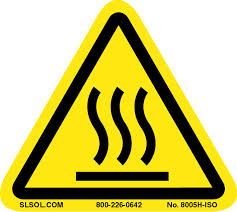
\includegraphics[width=\linewidth]{images/burn_hazard.jpg}
\end{wrapfigure}
\ \\
This icon is used to indicate a burn hazard.  Students should take care not to touch the surface or item that may cause burns.  Students should always treat the surface as though it is hot at all times.  Burn hazards can cause severe burns, bleeding, and possible loss of appendages.
\end{framed}
\newpage

\begin{framed}
\begin{wrapfigure}{L}{0.15\linewidth}

\includegraphics[width=\linewidth]{images/cut_hazard.jpg}
\end{wrapfigure}
\ \\
This icon is used to indicate a sharp tool or possible cutting hazard.  Students should take care in handling this tool or equipment.  Students should always treat the instrument as though it is very sharp.  This hazard can cause cuts, bleeding and possible loss of appendages.  
\end{framed}

\begin{framed}
\begin{wrapfigure}{L}{0.15\linewidth}

\includegraphics[width=\linewidth]{images/electrocution_hazard.jpg}
\end{wrapfigure}
\ \\
This icon is used to indicate an electrocution hazard.  Students should take care not to electrocute themselves when using that equipment.  Students should always treat the equipment as though it is live at all times.  Electrocution can cause burns, physical harm and even death.
\end{framed}

\begin{framed}
\begin{wrapfigure}{L}{0.16\linewidth}
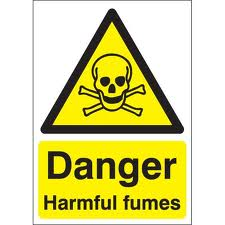
\includegraphics[width=\linewidth]{images/fumes_hazard.jpg}
\end{wrapfigure}
\ \\
This icon is used to indicate a fumes hazard.  Students should take care not to avoid these dangerous fumes and PPE equipment must be used.  Students should always treat the equipment as though it is live at all times.  Inhalation of dangerous fumes can cause illness, physical harm and even death.
\end{framed}

\part{M:2:I Policies}
% Student Conduct Poliicies
% This file needs to be included in a main LaTeX file

% Policy updated - 1/24/2017

\chapter{Student Conduct and Requirements}

All students enrolled at Iowa State University and are currently in good standing with ISU may join a M:2:I project or propose a project.  All students are invited and encouraged to be involved in Make to Innovate.  The program is managed by the Aerospace Engineering Department through the Make to Innovate Program Coordinator.  All policies and rules are therefore managed and enforced by the Make to Innovate Program Coordinator and the department.  Any questions or concerns with these rules should be made to the Make to Innovate Program Coordinator.  

\section{Student Code of Conduct}
Students in the M:2:I program represent M:2:I, the Aerospace Engineering Department, the College of Engineering and Iowa State University.  It is for this reason we expect students to adhere to a \index{code of conduct} both on campus and off campus.  Students that fail to adhere to these rules may receive a lower grade, a failing grade, or may be removed from the program.  In addition, these policies do not replace the Iowa State University Student Disciplinary Regulations, and some actions may fall under these regulations and associated disciplinary actions.  Any such action that falls under those regulations will be reported to the \index{Dean of Students Office} (DSO) and may have additional disciplinary action taken including and up to expulsion.  Students should read the Iowa State University Student Disciplinary Regulations and you can find these at this URL - \url{http://www.policy.iastate.edu/policy/SDR}  

The following are items that all students in Make to Innovate are expected to follow.

\begin{itemize}
\item All students must follow all signs posted in the M:2:I lab or any other M:2:I facility
\item All students must follow all lab monitor or lab technician instructions
\item All students must follow instructions from the M:2:I Program Coordinator or any other M:2:I faculty/staff
\item All students must follow instructions from their faculty adviser
\item All students must treat all fellow students with respect
\item All students must treat visiting members and members of the public with respect
\end{itemize}

Any case of misconduct will be reviewed by the M:2:I Program Coordinator and/or the Aerospace Engineering Department chair.  

\section{\index{Student Requirements}}
In order to be part of M:2:I, students must meet the following requirements.

\begin{itemize}
\item Must be in good standing with the University
\item Students must be enrolled in either AerE 294X or AerE 494X
\item A student must not be on academic probation
\item A student must be full-time status and must be on campus.
\item Students must have permission from the instructor
\end{itemize}

Students must be on campus or be taking the majority of their course load on campus.  Students are not permitted to take AerE 294X or AerE 494X while also on internship or Co-Op.  The Make to Innovate program is designed and can not be taken as a distance education course.

\section{\index{M:2:I Project Requirements}}
Teams in M:2:I must meet the following requirements in order to form a new team and to maintain the team status of ``in good standing'' with M:2:I.  Teams that fail one or more of these requirements may lose funding and/or membership in M:2:I.  It may also affect the teams grade for the semester in which they are enrolled.
\begin{itemize}
\item All teams must have 100\% of its active members enrolled in 294X or 494X.
\item All projects must have an approved charter on file with M:2:I.
\item If a team is requesting funding, an approved budget must be on file with M:2:I.
\item Teams must have a minimum of 3 students, at least one student must be enrolled AerE 494X.
\item Teams must not have more than 8 students including the team leader.
\end{itemize}

M:2:I is a program that is designed to compliment students academic achievements.  Therefore, we want our students to not only have fun in M:2:I but succeed academically as well.  If a student has a GPA lower than 2.5 or a team member is put on academic probation, they may not be active in M:2:I unless they have met with both their academic advisor and the M:2:I Program coordinator prior to signing up for M:2:I.  Both the academic adviser and the M:2:I coordinator must approve a student being involved in M:2:I before they are active in M:2:I.

% M:2:I Lab Policies

\chapter{Lab Policies}

\section{0620 Lab Space}
The Make to Innovate lab is located in 0620 Howe Hall.  It is shared space that is shared with M:2:I, AeroE Senior Design and on occasion other student organizations.  The 0620 Lab is also on the both the department and the College of Engineering tours.  This means that we often have guests that visit our lab.  The following policies are in place to ensure that everyone enjoys the lab and the lab is maintained and presentable not only to M:2:I groups but to visitors as well.

\section{Lab General Policies}
The lab is open to all students that are currently enrolled in AerE 294X or AerE 494X.  Other courses or organizations that has been approved by either the Aerospace Engineering Department or the M:2:I Program Coordinator may also use the space.  The space is also often on departmental, College of Engineering and other tours and often has guests that may visit the lab.

\subsection{Food and Drink}
Food in the Make to Innovate lab is not allowed at any time. Drinks are acceptable outside the safety glasses required zone and in the conference room.  All alcoholic beverages are off limits in the lab and on school property per ISU policy. Anyone caught having alcoholic beverages in the lab will be turned into the appropriate authorities.  A group may request to host an event in the conference and request to have food there.  These will be approved on a case by case basis.

\subsection{External Tools/Items}
Lab policy prohibits any tools, supplies, or items in general from being brought into the lab. This includes items intended for temporary use. All needed tools and most consumables will be supplied by the lab. If the has run out or does not carry a certain material/tools, an External Supplies Form must first be filled out and approved. This policy is in place to prevent items that are not lab supplies from being misplaced as well as ensuring that items that are being used in the lab are approved items. 

\subsection{In-Kind Donated Items}
The Make to Innovate Lab welcomes In-Kind donated items as these help to better the lab and quality of learning in the lab. In order to prevent confusion as to what is and is not lab property, donors must fill out the In-Kind Donation Form prior to donating any item to the lab.

\section{Lab Usage Policy}
Students that are using the lab must follow all signs, safety protocols, procedures and instructions from M:2:I Staff, Faculty and Lab Monitors.  Care must be taken that all students have taken all required training and understand that the lab must be used in a safe manor.  

\subsection{Trainings}
All students using the M:2:I lab must have completed the following trainings.  Three of the trainings are from Iowa State University's Environment Health \& Safety (EH \& S) website and the last one is on the Make to Innovate Blackboard page.

\subsection{Lab Personnel}
At least one lab monitor will be on duty at all times that the lab is open. Lab monitors will handle all questions that are not related to purchasing, budget or grades. If a student is unable to resolve an issue with a lab monitor, they should contact the M:2:I Program Coordinator to address any concerns.  Any issue involving grading of the course, purchasing or budget questions should go directly to the M:2:I Program Coordinator.  If a student has an issue with a lab monitor or any other M:2:I personnel, they should contact the M:2:I Program Coordinator immediately.  

\subsection{Lab Cleanup Policy}
Upon completion of an individuals work in the lab, the individual will be expected to clean up after themselves. Cleaning includes but is not limited to, cleaning up and returning tools to the tool crib, returning materials to their respective locations, vacuuming off all used equipment, and sweeping within the work area that the individual occupied.
\subsection{Access Policy}
Access to the M:2:I 0620 lab is a privilege and not a right.  To ensure the safety to our students and for the security of the tools, equipment and materials used, access to the lab is closely monitored and is limited to only students that have access to the space.
\section{Regular Hours}
Regular \index{lab hours} are posted near the lab entrance and online. Students are encouraged to make use of the regular lab hours as extended and after hours access is severely limited. The tool crib will only be open for checkout while a lab monitor is on duty and power tools may not be used without a lab monitor present.


\subsection{Extended Hours}
Extended hours may be granted at the discretion of Matthew Nelson. If your team is working in the lab and you know that you would like to stay late, please ask the lab monitor on duty at least an hour before closing. If your team needs short term extended access (weekends or before/after regular hours), fill out the extended access request form at least 3 days in advance and a lab monitor will contact you if they are able to accommodate you.
\subsection{After Hours Access}
Team leads will be granted after hours access to the lab via RFID. Other students may apply for after hours access in writing to Matthew Nelson only if absolutely necessary. No tools can be checked out and no power tools may be used without a lab monitor present.  No student may be in the lab when Howe Hall is closed.  Howe Hall is closed from midnight to 6 a.m. each day.  In addition, Howe Hall may be closed over certain holidays as well.

\section{Tool Policy}
All tools within the 0620 M:2:I lab are monitored and controlled through the M:2:I tool system.  This system allows us to track inventory and to ensure that all teams have equal access to the tools in the lab.  
\subsection{Training}
In order to check out tools, prior training must be completed. Training will be specific to the type of work being completed rather than for a specific tool. For example, foam working will require a single training program that covers the entirety of the foam tools as well as best practices. If the appropriate training has not been completed for the task a student wishes to do, then that student will not be allowed to use the tools required for that task.
\subsection{Consumables}
M:2:I groups may use lab consumables within reason.  Usage will be tracked by the lab monitors and be reported to Matthew Nelson.  Excessive usage may result in teams being charged for usage of these consumables.

Groups from outside M:2:I may not use lab consumables unless they have prior written approval from Matthew Nelson.  At this time M:2:I does not have the ability to charge outside entities.
\subsection{Tool Checkout}
Upon signing up for Make to Innovate and completing basic training, students will be issued an RFID card. This RFID card will connect to an internal database that keeps track of the training each student has completed. Tool checkout is accomplished by swiping their RFID card. If the tool’s training requirements have been met, then a lab monitor will then proceed to check out the tool to the student. It is then the student’s responsibility to ensure that the entirety of the tool is returned in good working condition.
\subsection{Disciplinary Action}
If a tool is returned and does not work or is missing components that were present upon checkout, a disciplinary system will be enacted. The first offense will be a warning and will be marked in the internal database. Additional offenses will be punishable by a fine to be payable to Make to Innovate to replace the tools or components. This fine will be deducted from the team’s budget. The fine will be assessed based off the dollar amount required to replace the tool or component. 
\section{Project Storage}
Each team will be issued a single locker in which they can store their project materials. All lockers are lab property and are subject to all lab policies. All project related materials must be stored in this locker and need to be labeled with the group’s name. The locker is to be locked at all times. No tools or chemicals of any kind are to be kept in group lockers. Tools will be supplied by the lab and can be obtained for use by following the tool checkout procedures. Chemicals that the lab provides or that are purchased by a group must be stored in the flammables locker that is in the tool crib. This is to prevent spills, leaks, and potential fire hazards. 
\subsection{Shelf Space}
In addition to the locker that is assigned to each group, additional shelf space can be obtained for project storage. This shelf space is primarily for storing large items that the group cannot readily fit in their provided locker space. Shelf space will be divided into 2 foot sections and will be allocated to groups who fill out the Additional Space Request form. The amount of space a team receives will be dependent upon the amount of space the group requested, the amount of space available, and the number of other teams that also need space. Space is not guaranteed and is ultimately up to lab monitors and Matthew Nelson to approve.
\subsection{Travelers}
All items are to be stored in either the group’s locker or on shelf space that has been allocated to them. However, if a project needs temporary storage for their project on a work table, they can do so by filling out a traveler form. Travelers are paper forms that must be attached to any item that is to be left outside of a group’s storage areas. These forms allow monitors and other groups know who the project belongs to, how to get a hold of them, and how long the project will be there. Travelers are a temporary form, and are not designed to be used for extended periods of time. The group must fill out all the information on the form and then turn it into a lab monitor. The lab monitor will then either approve or deny the request based on duration of the request, reason for the storage, and upon space that is currently available. Items left out without a traveler will be jailed. In addition to jailing, the first offense will result in a warning with repeated offenses requiring a written apology letter and an escalating grade or monetary penalty.
\chapter{Lab Resources}
0620 Howe Hall has a number of resources that are available to M:2:I students.  Some resources are also shared with other students and/or with the Aerospace Engineering Department.
\section{Computer Room}
The computer room is open to all students both from Make to Innovate as well as outside of the organization. Computer room hours are restricted to lab hours and will not be extended. When the lab closes, all persons using the computer lab will be required to leave regardless of the situation. The lab operates on a first come first serve basis, meaning there is no priority list for use of these computers.
\section{Conference Room}
The lab conference room is a space that has been set aside for use by M2I groups. Groups can set up recurring meeting times by filling out the M2I Conference Room Request form. This form is available online or you can pick up a copy from the lab monitors desk. The form must be turned in at least one day prior to the planned meeting. In order to see what time slots are available, check the Conference Room calendar at http://bit.ly/m2iconference. Forms must be turned into a lab monitor. Lab monitors will then check the available times and if the slot is available, they will add the group to the calendar. Requests are not final until they show up on the calendar.
\section{Laptop Usage}
The Make to Innovate lab has a supply of laptops that can be checked out for school use for both individuals as well as groups. These can be checked out through a lab monitor. In order to check out a laptop, an individual will have to present their Iowa State University ID card, which will be held until the laptop is returned. Once an individual has checked out a laptop, they are then fully responsible for the laptop until they have checked the laptop back into a lab monitor.
\section{Storage Room/Bulk Supplies}
Lab supplies will be stored in the storage room. This room will remained locked at all times and can be accessed via a lab monitor. Lab supplies can be used for a group's project, however each group's consumption will be monitored to avoid excessive use.
\chapter{0620 Safety Policy}
The M:2:I Lab Space is a multifunction lab and shop space that allows students to work on their projects in a safe environment.  The M:2:I Lab gives students the ability to design, build, test and learn from their projects.  Use of this lab space however is a privilege, and therefore students must follow all rules, policies and procedures or risk temporarily or permanent removal from the lab.

All students using the lab space must have the following trainings complete:

\begin{itemize}
\item EH\&S PPE Training
\item EH\&S Fire Training
\item M:2:I General Lab Training
\end{itemize}

Additional trainings for other tools in the lab may also be required.  Students that do not have these training completed will not be allowed to use the lab space or equipment.  For more information please see the M:2:I Training Manual.

\section{Student Conduct}
Students working in the lab must not work alone.  No student should be in the lab by themselves.  Working alone in the lab is a major safety concern as if something happens to that student, they would have no method to call for help.  

No horseplay is permitted at any time in the lab.  Students should never attempt to startle or surprise any person that is working in the lab.  Students are expected to maintain a professional environment at all times while working in the lab.

\section{Personal Protective Equipment}
While we have worked hard to make the 0620 lab space as safe as possible, hazards are still present in the lab when construction and other tasks are taking place.  Students can reduce their risk of injury by wearing the appropriate safety equipment.  Some \index{PPE} is required while others may be optional but are desired.  Students are ultimately responsible for their own safety.  The policies set forth here are to guide students on what the lab requires students to wear.  Training on safety equipment can be found in the M:2:I Training Manual.

\subsection{Dress Code}
Students working in the M:2:I Lab must follow the following \index{dress code}:

\begin{itemize}
\item No open sole shoes at any time
\item No loose clothing
\item No shorts or skirts
\end{itemize}

Students should expect to dress as though they are working with tools and equipment in the lab at all times.  

\subsection{Safety Glasses}
\index{Safety glasses} must be worn in designated safety glasses areas. Figure \ref{fig:0620_floor_plan} shows the floor plan of the 0620 lab space.  Areas in yellow must have safety glasses worn at all times.  No tools that require safety glasses may be used outside the designated areas.

\begin{figure}[ht]
\centering
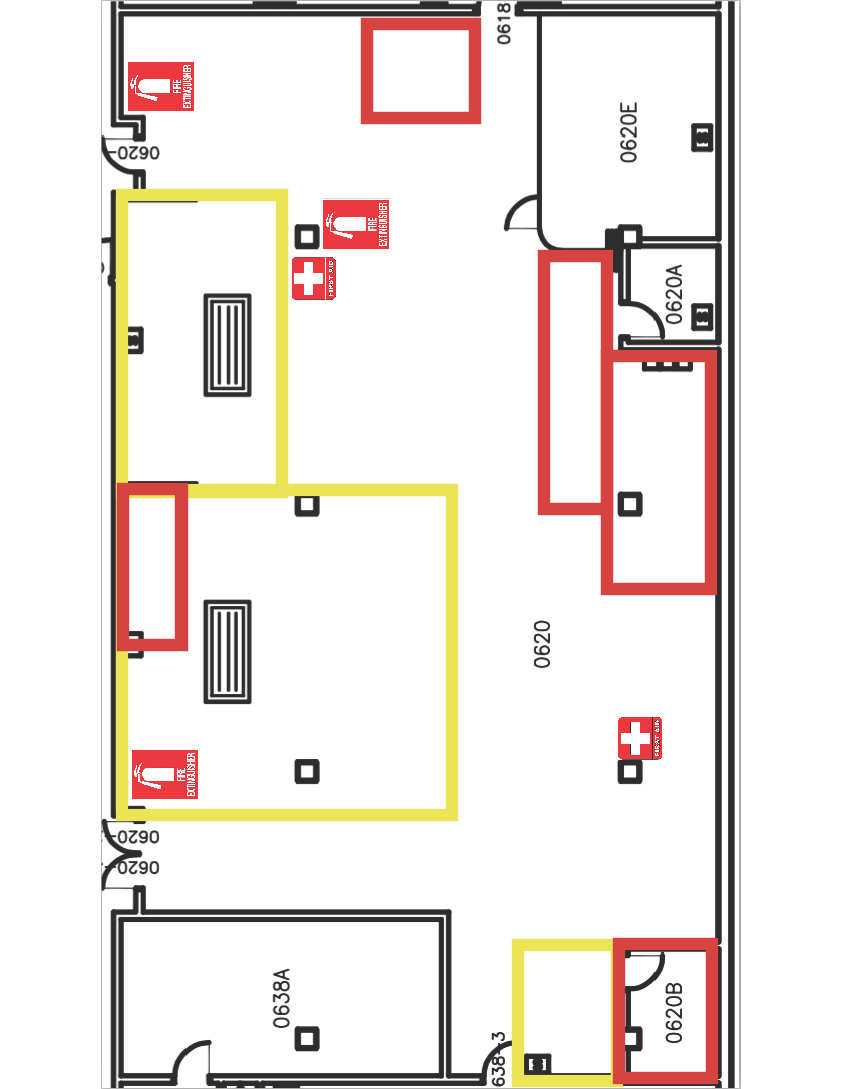
\includegraphics[width=5in]{images/0620_Floor_Plan.png}
\caption{0620 Floor plan with safety glasses and restricted areas marked}
\label{fig:0620_floor_plan}
\end{figure}

Safety glasses must be \index{ANSI Z87.1} approved.  Safety glasses must be marked with a Z87 as the minimum requirement and Z87+ is preferred for use the 0620 lab.  An example of the marking that should be shown is in Figure \ref{fig:ansi}.  Lightly tinted safety glasses may be used but fully tinted safety glasses are not permitted.  Students that wear prescription glasses may use those glasses only if the glasses are also ANSI Z87.1 approved and properly marked.  The appropriate side shields must also be installed and must also meet ANSI Z87.1 approval.

\begin{figure}[ht]
\centering
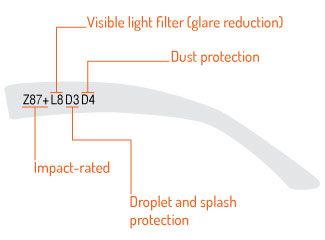
\includegraphics[width=4in]{images/ansi-z871.jpg}
\caption{Safety glasses with proper ANSI marking}
\label{fig:ansi}
\end{figure}

\subsection{Gloves}
The M:2:I Lab space has \index{nitrol gloves} that well suited for working with adhesives, paints and other materials that may cause chemical irritations to the skin.  These gloves  must be worn and the work surface must be protected when working with adhesives, paints or other solvents. Make sure you select the correct glove size for your hand so they are comfortable to use.

Leather or cloth gloves may be used if desired when working with wood or other materials.  However, these are not provided to students.  Use of gloves near \index{power tools} such as the \index{bansaw} or drill may cause a hazard if care is not taken to ensure the gloves do not get caught up in the machine.  For this reason, we leave the use of these gloves to the personal preference of the student using the machine.  Students however should consult either the M:2:I Program Coordinator or other faculty and staff if they have questions on what they should wear.  

\subsection{Masks}
The M:2:I Lab has \index{filtration masks} that are useful for filtering small and large particulates from the air when working.  Masks must be worn when sanding or working with aerosols. The masks that are provided are disposable and may only be used once per session.  Anytime that masks are required, safety glasses are also required to be worn.

\chapter{M:2:I Travel Policy}

\section{Introduction}
Make to Innovate supports projects that may need to travel.  Whether this travel is in Iowa, across the United States or abroad, M:2:I wants students to expand their knowledge by participating in activities and events that supports the M:2:I mission.  In order to support projects with their travel needs, M:2:I has established travel policies and procedures for all projects wishing to travel.  

These policies and procedures do not supersede any Aerospace Engineering, College of Engineering or Iowa State University policies and procedures.  Instead, these policies and procedures are meant to complement those procedures and provide students in M:2:I a mechanism to request such travel.  This policy and related procedures are designed to establish the relationship between M:2:I administrative staff and the requesting M:2:I project for the purpose of reducing risks and providing protection for all students participating in the travel.

\section{Policy Statement}
The Make to Innovate Travel Policy and procedures govern travel to reach an activity or event that is authorized by Make to Innovate and is an activity that is required by the project in order to full-fill a project objective, goal or milestone.  All Make to Innovate projects must comply with the requirements for travel as outlined in this policy and any other related procedures.

\section{Authorized Travel}
All travel by recognized M:2:I project must relate to the purpose of the organization and comply with the policies of the State of Iowa; the Board of Regents, State of Iowa; Iowa State University and Make to Innovate.  The ISU policy on Fleet Safety and Vehicle Use/Rental provides information for what is an approved vehicle use.  The purpose of the M:2:I project travel and transportation to and from the event is reviewed and authorized by the project's advisor, the M:2:I Program Coordinator, the Aerospace Engineering Department and the Office of Risk Management prior to travel. The M:2:I project leader must designate a member to serve as the trip coordinator who is responsible for completing trip information on the M:2:I Travel Authorization system.

\section{Eligible M:2:I Projects}
M:2:I projects eligible for travel and use of university vehicles must be in good standing with M:2:I and must not be probation.  Students going on travel must be current students and must be in good standing with Iowa State University.  Travel funding must be secured before requesting travel or the request will be denied.

\section{Forms}
The M:2:I Travel Request form must be completed to request travel for a M:2:I project.  Additional forms may be required dependent on the travel and at the discretion of the M:2:I Program Coordinator and/or Risk Management.

Students under the age of eighteen (18) must have the Waiver and Release of Liability form signed by their parents or legal guardian.

Students using personal vehicles for M:2:I projects travel must sign a Waiver and Release of Liability form and an Emergency Contact and Medical Information form acknowledging the risks involved in the travel activity and assuming responsibility for liability for themselves and any passengers traveling in their vehicle.


\section{Modes of Travel}
M:2:I Project leaders and their designated trip coordinator should consider transportation options and costs before planning a trip. M:2:I Project leaders will be asked to identify their mode of transportation, drivers (if applicable), participant(s) and/or commercial arrangements associated with their trip. Specific policies and procedures as they apply to different modes of transportation are outlined below.

\subsection{Vehicles}
To promote safe driving practices, all M:2:I projects must comply with the requirements for drivers and vehicle use rules outlined in this policy. For the purpose of this policy, vehicles include university vehicles; personal vehicles; vehicles rented, leased or hired by the university; or any vehicle in university control or custody for M:2:I activities.

\subsection{Driver Authorization}

Individuals requesting permission to drive vehicles for authorized M:2:I travel must submit a Motor Vehicle Record Check form to Transportation Services {MVR Check). This form is required to authorize a complete check of the driver's motor vehicle driving record. The individual's motor vehicle record must meet the following minimum qualifications:

\begin{itemize}
\item Driver must be at least 18 years old with the following exception:
\begin{itemize}
\item Drivers of large passenger vans or vehicles towing trailers must be 20 years old and must successfully complete the Transportation Services Large Passenger Van Driving Class.  See Section
\end{itemize}
\item Driver must have a valid U.S. driver's license for the vehicle being driven with the appropriate classifications, restrictions and endorsements.
\item Driver must satisfactorily complete a motor vehicle record check every six months (See Section Driving Standards section below).
\item Driver must agree to operate the vehicle in a safe and prudent manner.
\end{itemize}

Drivers for M:2:I travel must be M:2:I students, or M:2:I Faculty or Staff members.  Student drivers must be members of the project and who are currently enrolled as ISU students and in good standing.  When submitting a request the M:2:I Program Coordinator must used as the contact person.

\subsection{Driving Standards}

Driving privileges for individuals will be denied or revoked if a driver's past twelve-month driving record indicates any of the following:

\begin{itemize}
\item Two citations for a moving violation within the last 12 months.
\item Two accidents within the last 12 months where the driver was at fault or contributory. The definition of "at-fault accident" for this policy means an accident in which the driver is determined to be 50 percent or more responsible for the accident.
\item One accident where the driver was at fault or contributory and one moving violation within the last 12 months.
\item Any citation for blood alcohol content within the last 12 months. Cases not yet resolved in the courts will be considered grounds for temporarily denying permission to drive a university vehicle.
\item A licensing requirement for specialized motor vehicle insurance (i.e., SR) to operate a vehicle.
\item Conviction for reckless driving, driving with a suspended license, hit and run, leaving the scene of an accident, license suspension or other crime(s) that results in license suspension.
\item Conviction or charges pending due to a violation of statutes that affects his/her driver's license, or who has his/her driving privileges suspended, revoked, or barred for violating such statutes including, but not limited to, Operating While Intoxicated, vehicular homicide or habitual violations, or any driving offense punishable as a felony.
\end{itemize}

Individual drivers approved to drive university vehicles for authorized M:2:I travel must notify the M:2:I Program Coordinator and the Office of Risk Management when their driver's license is suspended, revoked, canceled or the driver is otherwise prohibited from operating a university motor vehicle. top

\subsection{Rules and Criteria - All Vehicles}

Passenger Authorization:

\begin{itemize}
\item Authorized passengers include students of the M:2:I project, university employees, or authorized volunteers and are directly involved with the M:2:I program or project.  All passengers must be identified in the M:2:I Travel Authorization system prior to departure.
\item Unauthorized passengers are prohibited in university vehicles. Examples include M:2:I project members not listed on the passenger list, spouses, children or other family members, friends, neighbors or the general public. Unauthorized passengers are not covered by the Regents institutions' insurance.
\end{itemize}

In extenuating circumstances, a request for authorization for passengers otherwise considered unauthorized must be submitted in writing and approved by the Office of Risk Management or Recreation Services (for Sports Clubs) before travel occurs.
Vehicle Occupancy: The maximum number of people in any vehicle must not exceed the number of seatbelts in the vehicle.

In addition the following policies must be observed at all times:

\begin{itemize}
\item All vehicle occupants must wear seat belts at all times while traveling.
\item Transporting people in the bed of a pick-up truck is not allowed on public roads.
\end{itemize}

\subsection{Driving Rules}
The following driving rules must be observed at all times.  Failure to observe these rules may result in revocation of driving privileges.  

The number of drivers required may vary depending on the distance and duration of the trip and must figured in the travel planning.  Drivers are also expected to follow the rules below:

\begin{itemize}
\item Each driver is allowed to drive a maximum of 4 continuous hours followed by a minimum 2-hour break.
\item Each driver is permitted to drive a maximum of 10 hours over a 24-hour period.
\item One person must be in the front passenger seat and awake at all times to assist with navigation and trip safety such as making sure the driver remains alert.
\item Drivers must obey traffic laws and regulations, including posted speed limits.
\end{itemize}

Drivers must abide by university policies and any applicable federal or state regulations that govern individual actions including, but not limited to, ethical behavior, confidentiality, financial responsibility, alcohol and drug use.  No alcoholic beverages or beverage containers (open or closed) are allowed in or around the vehicle. Consumption of alcohol by drivers and passengers is prohibited at all times during the travel and event that the M:2:I project is participating in.  

\subsection{Transporting Hazardous Materials}

The unauthorized transportation, use or storage of any hazardous materials is prohibited. In extenuating circumstances, a request for authorization for transporting hazardous materials must be submitted in writing and approved by the Department of Environmental Health and Safety and the Office of Risk Management before travel occurs. In addition, the Office of Risk Management and the M:2:I Program Coordinator must review and authorize any project activity that involves the use of hazardous materials.

\subsection{Firearms, Weapons and/or Explosives}

The unauthorized transportation, use or storage of any firearms, weapons and/or explosives is prohibited. In extenuating circumstances, a request for authorization for transporting firearms, weapons and/or explosives must be submitted in writing and approved by the Office of Risk Management and the M:2:I Program Coordinator. In addition, the Office of Risk Management and M:2:I Program Coordinator must review and authorize any M:2:I project activity that involves weapon or gun use.

\subsection{Cell Phones and Other Communication Devices}

The use of cell phones and other communication devices such as walkie-talkies while driving is hazardous. Only hands-free units may be used while driving. Drivers are required to stop and park the vehicle to use any other devices.  2-way communication devices such as amateur radio equipment may only be used by the passengers in the vehicle.  Cell phones and other distractions should be kept in a minimum to avoid distractions to the driver.

\subsection{Travel Restrictions}

Travel is not allowed between 1:00 a.m. and 5:00 a.m. on any day.  There are no exceptions to this rule.  In the event of adverse weather or other factors that affect the ability to drive safely, drivers are expected to use good judgment and take appropriate safety measures in observance of travel warnings as issued by the highway safety authorities or weather advisory services.

No items may be transported on the roof of a vehicle.  Rear seats of university vans will not be removed to accommodate luggage without approval from Transportation Services.  Luggage must be dispersed evenly throughout large passenger vans to equalize the load.  When using large passenger vans (12 to 15-passengers) on extended trips, Transportation Services may require a trailer to safely accommodate luggage.

\subsection{Trailers}

Trailers owned by Transportation Services must be used if available.
Transportation Services must approve the use of all commercially rented, privately owned, manufactured, home-made or donated trailers and has the authority to deny the use of any trailer.  Transportation Services must inspect all trailers after connection to the vehicle.  University owned trailers may be pulled only by university owned vehicles.

\section{University Vehicles}\label{ISU_Vehicles}

University vehicles may be used only for official M:2:I travel. All M:2:I projects must comply with the Iowa State University Fleet Safety policy as well as all federal or state regulations that govern related actions including, but not limited to, those of drug and alcohol use, ethical behavior, confidentiality, harassment and financial responsibility. Operating a university vehicle is a privilege. The M:2:I Program Coordinator in conjunction with Transportation Services and/or the Office of Risk Management have the authority to approve or deny any request for the use of university vehicles.

Iowa State University vehicles are easily identifiable. Common sense must be used and consideration must be given to public perceptions of how vehicles are operated and where they are parked. The Iowa Code does not permit personal use of university vehicles and individuals who use vehicles for personal purposes are subject to corrective action or disciplinary measures according to the severity of the infraction and are potentially liable for accidents, injury and damages that occur during unauthorized use.

\subsection{Large Passenger Vans and Vehicles Towing Trailers}

M:2:I projects may be approved to use Iowa State University Transportation Services' 12- and 15-passenger vans for trips with nine to fifteen passengers and/or vehicles towing trailers. Projects may not rent 12- or 15-passenger vans from commercial rental companies or use personal 12- or 15-passenger vans for authorized M:2:I travel.

Due to their unique handling characteristics, drivers of large passenger vans and vehicles towing trailers must be at least 20 years old. In addition, driver training as described below is required.

\subsection{Driver Training}

All drivers of 12- and 15-passenger vans or vehicles towing trailers must complete the Large Passenger Van Driving Class offered by Transportation Services. The Large Passenger Van Driving Class is a two-hour classroom session that covers handling characteristics and defensive driving techniques for 12- and 15-passenger vans.

Each driver must also show behind-the-wheel driving competency by driving a large passenger van with a trailer attached. Competency is determined by the Transportation Services instructor. Behind-the-wheel training will be scheduled after the classroom training is completed.

Each driver must have a record of successful completion of both the classroom and the hands-on, behind-the-wheel training before picking up the keys for a vehicle.  Training records will be kept on file with Transportation Services.

\subsection{Rules and Criteria - University Vehicles}\label{ISU_Vehicle_Criteria}

The following is additional rules and criteria pertaining to ISU University Vehicles.

Smoking is not allowed in Iowa State University vehicles.  All drivers are expected to properly safeguard university vehicles. If it is determined that a vehicle is at substantially higher risk of theft or damage due to a lack of reasonable precautions by the driver or the M:2:I project; the M:2:I project will be notified by the M:2:I Program Coordinator to implement measures to correct the misuse. If the misuse is not corrected within a reasonable time, the M:2:I project may be required to forfeit use of the vehicle and return the vehicle to Transportation Services.  The M:2:I project may also be banned from using ISU vehicles in the future.

All drivers are expected to properly safeguard university vehicles. If it is determined that a vehicle is at substantially higher risk of theft or damage due to a lack of reasonable precautions by the driver; the M:2:I project will be notified by the M:2:I Program Coordinator to implement measures to correct the misuse. If the misuse is not corrected within a reasonable time, the M:2:I project may be required to forfeit use of the vehicle and return the vehicle to Transportation Services.

University vehicles may not be taken into Mexico or Canada without the prior written consent of the Office of Risk Management. Travel into Mexico requires the purchase of Mexican auto insurance and must be arranged through the Office of Risk Management. In addition, the Office of Risk Management must review and authorize any student activity that involves travel to Mexico or Canada.

University vehicles may be driven to a private residence and parked overnight when travel is scheduled to depart early in the morning. Other than short-term travel (i.e. a day or less), private or public transportation should be used to access airports, as it is neither an economical nor effective use of university vehicles to leave them in an airport parking lot.

\section{Personal or Privately Owned Vehicles}

M:2:I projects should minimize the use of personal vehicles for M:2:I-related travel. When a personal vehicle must be used for M:2:I travel, the driver assumes all liability associated with the trip. Drivers and passengers must comply with the M:2:I Travel policy Driving Authorization, Driving Standards and vehicle use Rules and Criteria - All Vehicles. Students using personal vehicles for M:2:I travel must sign a Waiver and Release of Liability form and Emergency Contact and Medical Information form acknowledging the risks involved in the travel activity and assuming responsibility for the liability for themselves and the passengers traveling in their vehicle.

\section{Commercial Travel}
M:2:I projects who use commercial transportation for travel related to M:2:I travel must comply with all university regulations pertaining to commercial travel and the rules of the carrier. This applies to domestic as well as international travel.

\subsection{Air Travel}

Scheduled commercial flights are the most closely regulated and safest form of travel. M:2:I projects who choose other types of flights, such as charters or private planes, must contact the Office of Risk Management regarding contractual agreements and insurance provisions.

\subsection{Chartered Bus or Hired Vehicle}

M:2:I projects may request the use of university contracts for chartered bus or hired vehicle services by making a request to the M:2:I Program Coordinator.

\subsection{Rental Vehicle}

M:2:I projects must rent university Transportation Services vehicles for travel originating in Ames. M:2:I projects starting travel from another location and needing to rent a vehicle commercially must contact the M:2:I Program Coordinator prior to making arrangements.

\section{International Travel}
International travel by M:2:I projects requires extensive planning and preparation. M:2:I projects that wish to travel outside of the United States must complete information in the M:2:I Travel Authorization system and submit it to the M:2:I Program Coordinator at a minimum of six months prior to travel for review and final approval.

\section{Special Circumstances}
Any use of university owned vehicles that involves specific hazards (i.e., HABET Balloon chase, MAVRIC competition, CySLI rocket transportation, etc.) must be reviewed and approved by the M:2:I Program Coordinator and may require additional review from Risk Management.  All requests for exceptions to this policy or any changes to an approved travel itinerary must be submitted to the M:2:I Program Coordinator for approval prior to departure.  The M:2:I Program Coordinator in conjunction with the Aerospace Engineering Department and/or Risk Management will review all special circumstance requests and have the authority to approve or deny any request.

\section{Sanctions}
Failure to comply with any M:2:I Travel policies and procedures may be subject to disciplinary action from the M:2:I Program Coordinator, and/or the Office of Student Conduct disciplinary measures. In addition groups may have travel authorization revoked and may be placed on probation status within M:2:I.  Finally, addition actions may occur that may affect students final grade within the course.

\chapter{Travel Authorization Procedure}

The M:2:I Travel Policy and Procedures for M:2:I projects govern travel for activities or events that are sponsored and authorized by M:2:I.  Travel authorization requests must be submitted and approved prior to travel so the M:2:I staff can properly manage liability issues for student travel.  All forms for travel authorization can be found on the M:2:I Sharepoint site.

\section{Checklist for Travel Authorization}

Checklist for completing your M:2:I Travel Authorization Request:

\begin{itemize}[label={\checkmark}]
\item Click "Add a New Trip" above
\item Search the name of your M:2:I project
\item Complete the "General Information" as completely as possible.
\item Complete all "Travel Information" as completely as possible.
\item Complete all "Lodging Information" as completely as possible.
\item Complete all "Funding Information" as completely as possible.
\item Complete the Itinerary as completely as possible.
\item Complete all "Student Information" as completely as possible.
\item Click "Submit"
\end{itemize}

Once submitted your application will be reviewed by the M:2:I Program Coordinator and any other departments as needed.  Missing information will often delay and may result in your application being denied.  Ensure you have all information provided to help in speeding up the process.  The M:2:I Program Coordinator may request that a special meeting be called in order to get additional information.

In order to use university vehicles, you meet all requirements for using a university vehicle as outlined here and any additional requirements outlined from ISU Transportation.

\subsection{Updating the form}
M:2:I Projects may update their form if needed.  Please note that any update to the form will automatically trigger the need for re-authorization from the M:2:I Program Coordinator.  The list of student going may be updated or changed up to 4 weeks prior to travel.  

M:2:I project travel must relate to the purpose of the project and comply with the policies of the Board of Regents, State of Iowa, and Iowa State University. The purpose of M:2:I project travel and transportation to and from the event will be reviewed and authorized by the M:2:I Program Coordinator and other departments as needed. 

\subsection{Timeline for consideration}

All M:2:I projects that are traveling within the State of Iowa and doing so for an activity or event that will be 24 hours or less must submit an authorization at least 1 week in advance of the time of departure.  If an activity is weather dependent, M:2:I projects should submit a request 1 week in advance and may make changes up to 48 hours in advance of the time of departure.  These requests will typically be reviewed and approved within 48 hours but may take longer if needed or if the form is not completely filled out.

All M:2:I projects that will be traveling outside the State of Iowa for an activity or event that will be 24 hours or less must submit an authorization form at least 2 weeks in advance of the time of departure.  If an activity is weather dependent, M:2:I projects should submit a request 2 weeks in advance and may make changes up to 48 hours in advance of the time of departure.  These requests will typically be reviewed and approved withing 48 hours buy may take longer if needed or if the form is not completely filled out.

All M:2:I projects that will be traveling either within or outside the State of Iowa for an activity or event that will requires any overnight stay must be submitted at least 6 weeks in advance of the time of departure.  Changes to the form may be allowed up to 2 weeks prior to the time of departure.  These requests will typically be reviewed and approved within 1 week.  Additional time may be required depending on the nature of the travel.  This time-line also allows for time to make vehicle and hotel accommodations.

All M:2:I projects that will be traveling outside of the United States for an activity or event must be submitted at least \emph{6 months} in advance of the time of departure.  International travel requires additional permissions from the university which requires extra time.  In addition, additional time is required for securing all necessary paperwork for students that are traveling abroad.  Iowa State University has strict rules on international travel and some locations may not be accessible to studnets for travel.

\section{Trip Coordinator Responsibilities}
The M:2:I Project Leader must designate a member of the travel party to serve as the Trip Coordinator. The Trip Coordinator is responsible for submitting travel authorization requests through the M:2:I Sharepoint Site for each trip. Trip Coordinators must travel with the organization and act as liaison for their M:2:I project during the approval process and on the trip. The Trip Coordinator should confirm receipt of appropriate travel documents with M:2:I faculty and staff. When necessary, the Trip Coordinator may need to meet with staff to review and evaluate the completed M:2:I travel authorization information.

When using a 15-passenger van or a vehicle towing a trailer, the Trip Coordinator must ensure that drivers for the trip have completed Large Passenger Van training. Drivers who need to complete this training must contact Transportation Services and allow for enough time to register for and complete the next available class. These classes are available only through Transportation Services and are usually offered monthly.

\chapter{Event Policy}
Events are any activity that takes place either on or off campus that involves your team.  The only event that is excluded from this is weekly team meetings.  In addition, if the event takes place off campus, even in the Ames, IA area, a travel form must also be filled out.  The following is a list of examples.

\begin{itemize}
\item
Doing an outreach demonstration at a public school
\item
Traveling to a location to do a test flight
\item
Presenting a paper at a conference
\end{itemize}

Events must be pre-approved and if travel is required, that must be approved as well.  Teams are required to give a minimum of 48 hours notice before the event.  Teams are encouraged to provide as much notice as possible.  If the event requires approval from ISU’s Risk Management, there may be a delay in approving the event.  Always consult with the M:2:I Program Coordinator if you have a question on the time needed or if additional requirements are needed.

Some events that a team wishes to do may be dependent on things such as weather that is beyond the control of the team.  In these cases, a team may request am event window.  For these, a window of time will be granted with a maximum window of 1 week.  Teams may then use the best day and time for their event.  If no day or time works within the window, the team will be required to request another event window.
\part{M:2:I Training}
%General Lab Training
% Updated 2/11/2017

\chapter{General Lab Safety}

This chapter will cover basic tools and general information of the 0620 Lab Space also known as the M:2:I Lab  This document will cover some of the basic lab rules, procedures and information that all students should know in order to use the lab.  It will also cover some of the basic tools available to students.  Students should take the M:2:I General Lab Quiz on blackboard after they have read this training.

\section{Introduction}

The Make to Innovate Lab space offers a number of equipment and services that are available to students to use while working on their Make to Innovate (M:2:I) projects.  This includes the following:

\begin{itemize}
\item Electrical construction and diagnostic
\item Basic metal working
\item Basic wood working
\item Foam cutting and shaping tools
\item 3D Printers
\item Tabletop CNC machine
\end{itemize}

These tools and equipment are only accessible to students that are currently enrolled in the Make to Innovate program and currently assigned to an active and authorized project within M:2:I.  All other students must receive written permission from the M:2:I Program Coordinator.

Not all equipment in the lab can be used by students.  Some equipment, such as the 3D printers, and CNC machine can only be used by an authorized personnel.  Contact a lab monitor or the program coordinator if you need to use this equipment.  Additional costs may apply and can be charged to your project account.

Students wishing to use the 0620 lab space and any of the tools in the space must complete the following training:

\begin{enumerate}
\item Fire Safety and Extinguisher Training course
\item Personal Protective Equipment course
\item M:2:I General Lab Training
\end{enumerate}

Optionally students may take the EH\&S Shop Safety training.  This training provides some basics on shop safety and usage of tools.  However, the M:2:I General Lab Training will also cover many of the same things covered by the EH\&S Shop Safety Training.

These EH\&S training courses can be found at \url{http://www.ehs.iastate.edu/my-eh-s/training}. From there, click on ISU Login and enter your Iowa State login information. Then navigate to the Course Catalog page, which can be found on the left hand side bar. Type in the course name and click the Launch button to take the training. When completed, bring a printed copy of your completion certificates to the lab monitor on duty.  If you have a problem with the EH\&S website, please contact EH\&S.

Additional training may also be required in order to use certain tools and lab equipment.  Use of the electronics bench and foam cutter both require additional training and a quiz that needs to be passed by the student.  The foam cutter training can be found in Chapter \ref{foam_training} and the basic electronics training can be found in Chapter \ref{basic_electronics}.

\section{Hazards}
While we have taken many precautions to make the M:2:I Lab as safe as possible, students must still be aware that there are hazards in the lab.  With the proper training, personal protection equipment and care these hazards can be minimized and the impact to the student should be small.  However, students must always be aware that these hazards exist.  

\subsection{Electrocution}
\begin{framed}
\begin{wrapfigure}{L}{0.15\linewidth}

\includegraphics[width=\linewidth]{images/electrocution_hazard.jpg}
\end{wrapfigure}
\ \\
This lab space offers tools used for electrical testing and prototyping as well as power tools. All of these can potentially cause electrocution if improperly used. When using electrical equipment with power cords, always inspect the cords for damage prior to use. Never attempt to repair a damaged cord.
\end{framed}
Report any damaged cord or potential hazard to a lab monitor immediately. Never use a cord that is frayed or damaged as this can lead to electrocution.  Always ensure that when plugging in equipment, the plug is fully inserted into the outlet and has a snug fit. If the plug is equipped with a ground plug, the plug must still be in tact and must not be damaged.  Cords that aren't securely plugged in present a potential electrocution hazard. 

Extension cords may only be used for \emph{temporary} use.  Extension cords must be rated for the amperage the equipment requires.  Power strips may not be used for any power tool.  Use of power strips for low power applications is permitted.  When using tools or instruments that have specific training requirements, always complete the training and familiarize yourself with the operating procedures to reduce the risk of shock.

The electrical workbench has several bench power supplies that can supply both high voltage and high current.  Proper precautions must be observed to ensure to minimize risk to the user.  Additional information on the power supplies will be covered in Section \ref{power_supply}

\subsection{Burns}
\begin{framed}
\begin{wrapfigure}{L}{0.15\linewidth}
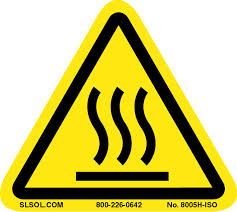
\includegraphics[width=\linewidth]{images/burn_hazard.jpg}
\end{wrapfigure}
Several tools in this lab space utilize heat in order to perform their designated task. Wearing gloves that are heat resistant when handling hot objects will help to reduce the risk of burns. Always be familiar with the safety and operating procedures of the tool being used in order to minimize burn risks. 
\end{framed}
Always be aware of your surroundings and others while working with hot tools and materials. If you are unsure how to use a tool, seek help from a lab monitor.  Some tools, such as the soldering irons, require additional training as well.

\subsection{Fumes}
\begin{framed}
\begin{wrapfigure}{L}{0.16\linewidth}
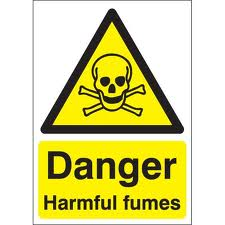
\includegraphics[width=\linewidth]{images/fumes_hazard.jpg}
\end{wrapfigure}
\ \\
Fumes may be present in this lab space. The most common sources will be from soldering and the various chemicals being used in the lab such as adhesives. Fumes have the potential to cause respiratory and ocular damage if not properly managed. Always read chemical labels before use. Always use a vent hood when dealing with volatile chemicals or items that can cause harmful fumes.
\end{framed}

Students must wear the appropriate PPE equipment when working with any chemical that poses a health risk.  If at any time you are uncertain what PPE should be worn, either consult with the MSDS sheets for that chemical or talk to a Lab Monitor or the Program Coordinator.  

\subsection{Chemicals}
Several chemicals may be in use in the lab and chemicals have the potential to cause injury from mild skin and eye irritation to severe burns and potentially death. In order to minimize this risk, be familiar with the chemical prior to use. Read and follow all safety information listed on the chemical. Always use a proper vent hood when dealing with chemicals that create harmful fumes.  Proper PPE equipment must also always be used when appropriate.  

\subsection{Cuts}
\begin{framed}
\begin{wrapfigure}{L}{0.15\linewidth}

\includegraphics[width=\linewidth]{images/cut_hazard.jpg}
\end{wrapfigure}
\ \\
Many of the tools in the lab can lead to cuts, both minor and severe if improperly used. Having the appropriate training that each tool requires is the best way to minimize the risk of cuts. 
\end{framed}
Always make sure that your immediate surroundings is cleared of potential hazards and other people before using cutting tools as this helps reduce the risk of injury to both yourself and others. Always cut away from yourself and bystanders. Don’t wear loose fitting clothing as this can be caught in the cutting tool and cause injury. 

\section{Safety}
Safety is our top concern in the Make to Innovate lab.  We want our students to be able to work on their projects in a safe and clean environment.  Because of this, we require all students to take the EH\&S trainings that cover personal protection equipment and fire safety and the M:2:I General Lab Training.  These courses contain a majority of the basic safety measures for the lab space and is often a requirement for other lab spaces on the campus of ISU. Addition signs have also been placed within the lab that relates to a specific risk or PPE that must be worn.  Read and become familiar with these regulations. 

There are two First aid kits in the lab that can address minor cuts, burns and irritations.  You should become familiar with the locations of these kits. Fire extinguishers are also near the exits of the lab and near the electronics area. Please refer to Figure \ref{fig:0620_floor_plan} that has a map of key safety features of the lab.

\subsection{Basic Safety Rules}
The lab has a set of basic safety rules that all students, faculty, staff and visitors should know.  All of these rules are also posted in the lab to remind everyone and inform visitors on these basic rules.  The following is the basic safety information that all persons in the lab need to know.

\begin{itemize}
\item No open sole shoes are allowed at any time
\item No loose jewelry or clothing is allowed at any time
\item Long pants must be worn at all times
\item Safety glasses must be worn in all designated areas
\item All signs posted must be adhered to at all times
\item Long hair must be securely pulled back
\end{itemize}

These basic rules apply to all those in the lab.  This includes all M:2:I students, faculty and staff and all visitors to the lab space.  If a person is caught that is not following theses rules, they will be asked to leave the lab or correct the error.

\section{Emergency procedures}
It is important to know the emergency procedures of the lab.  The lab has this information posted on signs near the exits of the lab as well as the evacuation routes.  A copy of this sign is also shown in Figure \ref{fig:Emergency_Response}. Please note that 0620 is also a tornado shelter in the event of a tornado.  In addition to the emergency signs, you need to familiarize yourself with the following.
\begin{itemize}
\item Know where all safety signs and emergency information is in the lab,
\item Know where all safety equipment is located,
\item Know the location of the fire extinguishers and first aid kits in the lab
\end{itemize}

\begin{figure}[ht]
\centering
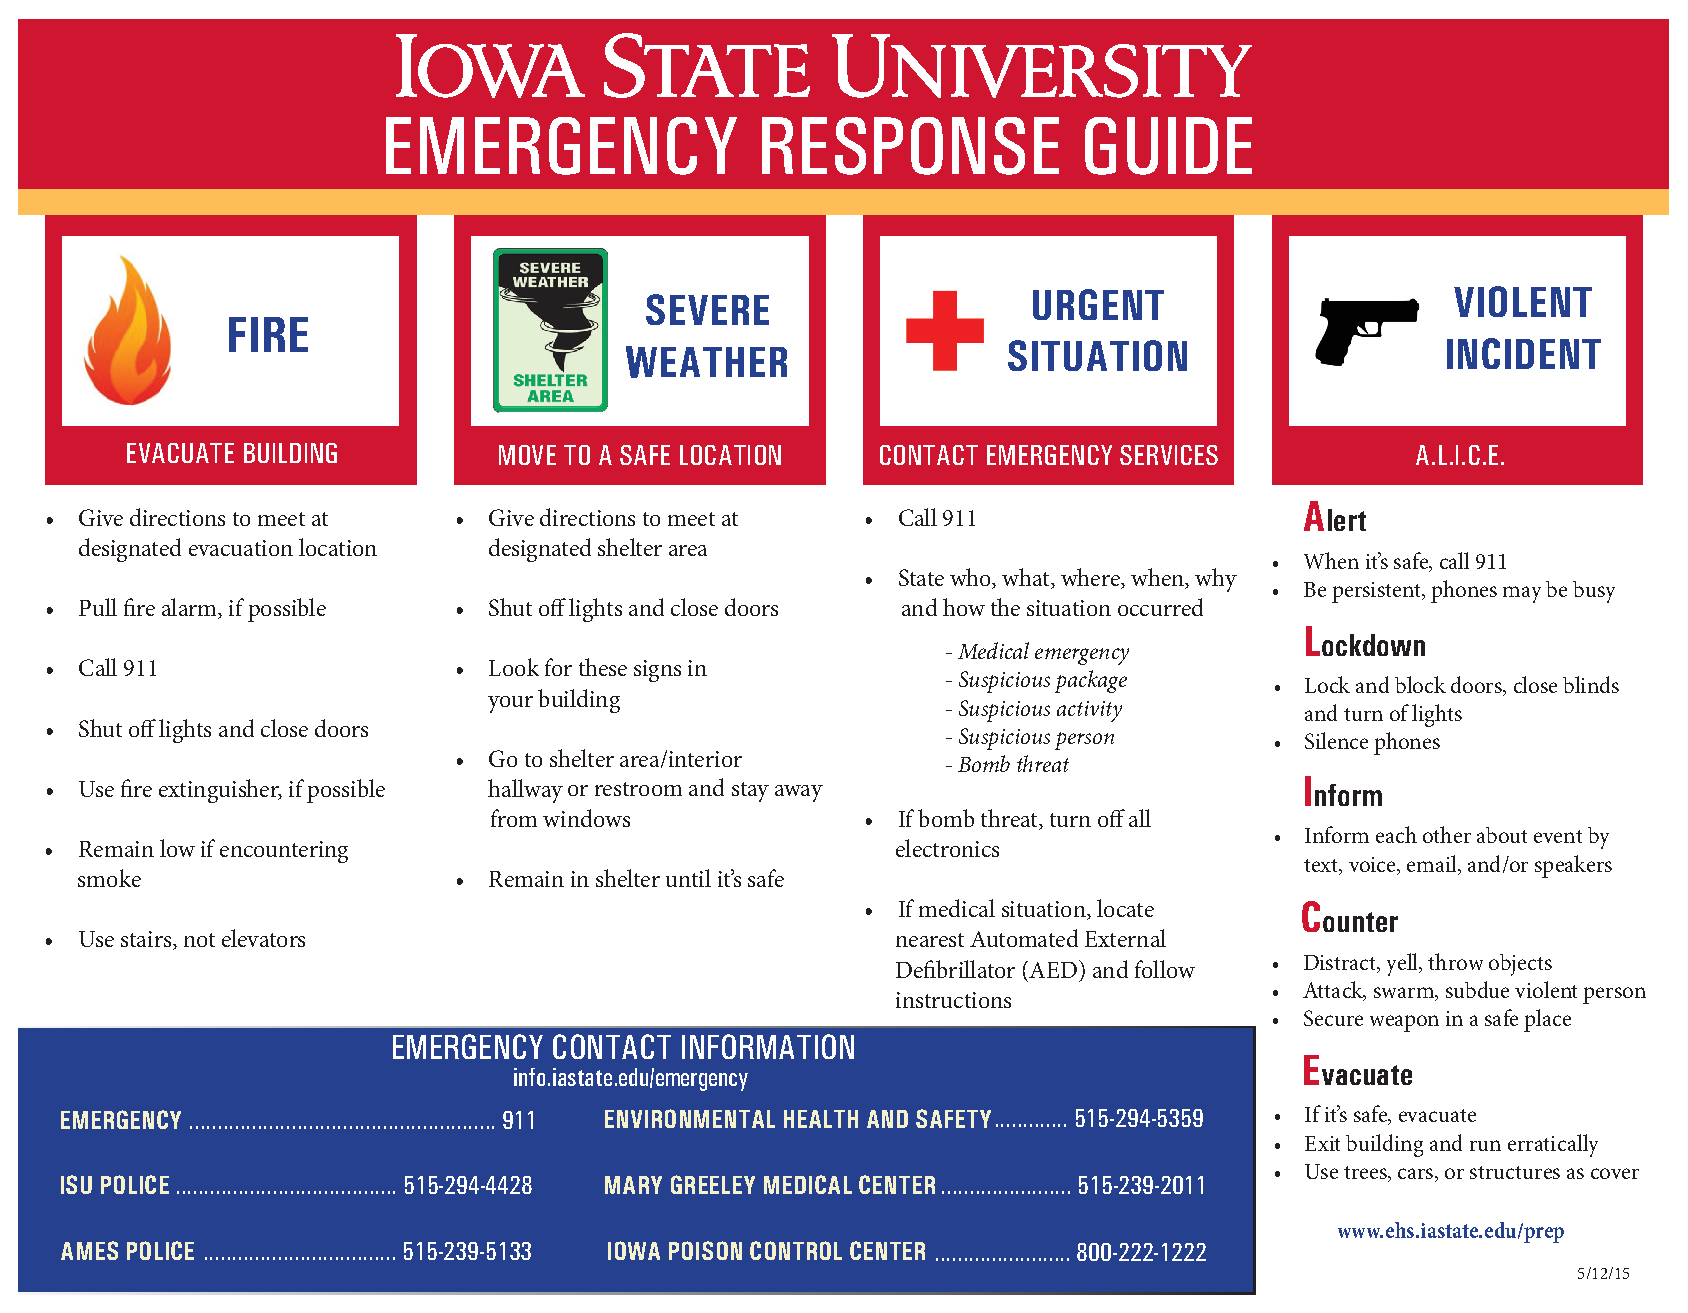
\includegraphics[width=6in]{images/EmergencyPoster.pdf}
\caption{ISU Emergency Response Guide Poster}
\label{fig:Emergency_Response}
\end{figure}

\subsection{Emergency Evacuation and Procedures}
In the event of a fire or other emergency students will be asked to leave Howe Hall in a safe and orderly manor.  Personnel should evacuate using the route indicated in Figure \ref{fig:Evac_map}.  In the event that the fire alarm has been activated, all personnel must evacuate the building immediately as per Iowa Law and ISU policy.  Even if it is suspected the alarm might be false, everyone must evacuate.  The building is only safe to return to when emergency responders have deemed it safe to enter the building again.

\begin{figure}[ht]
\centering
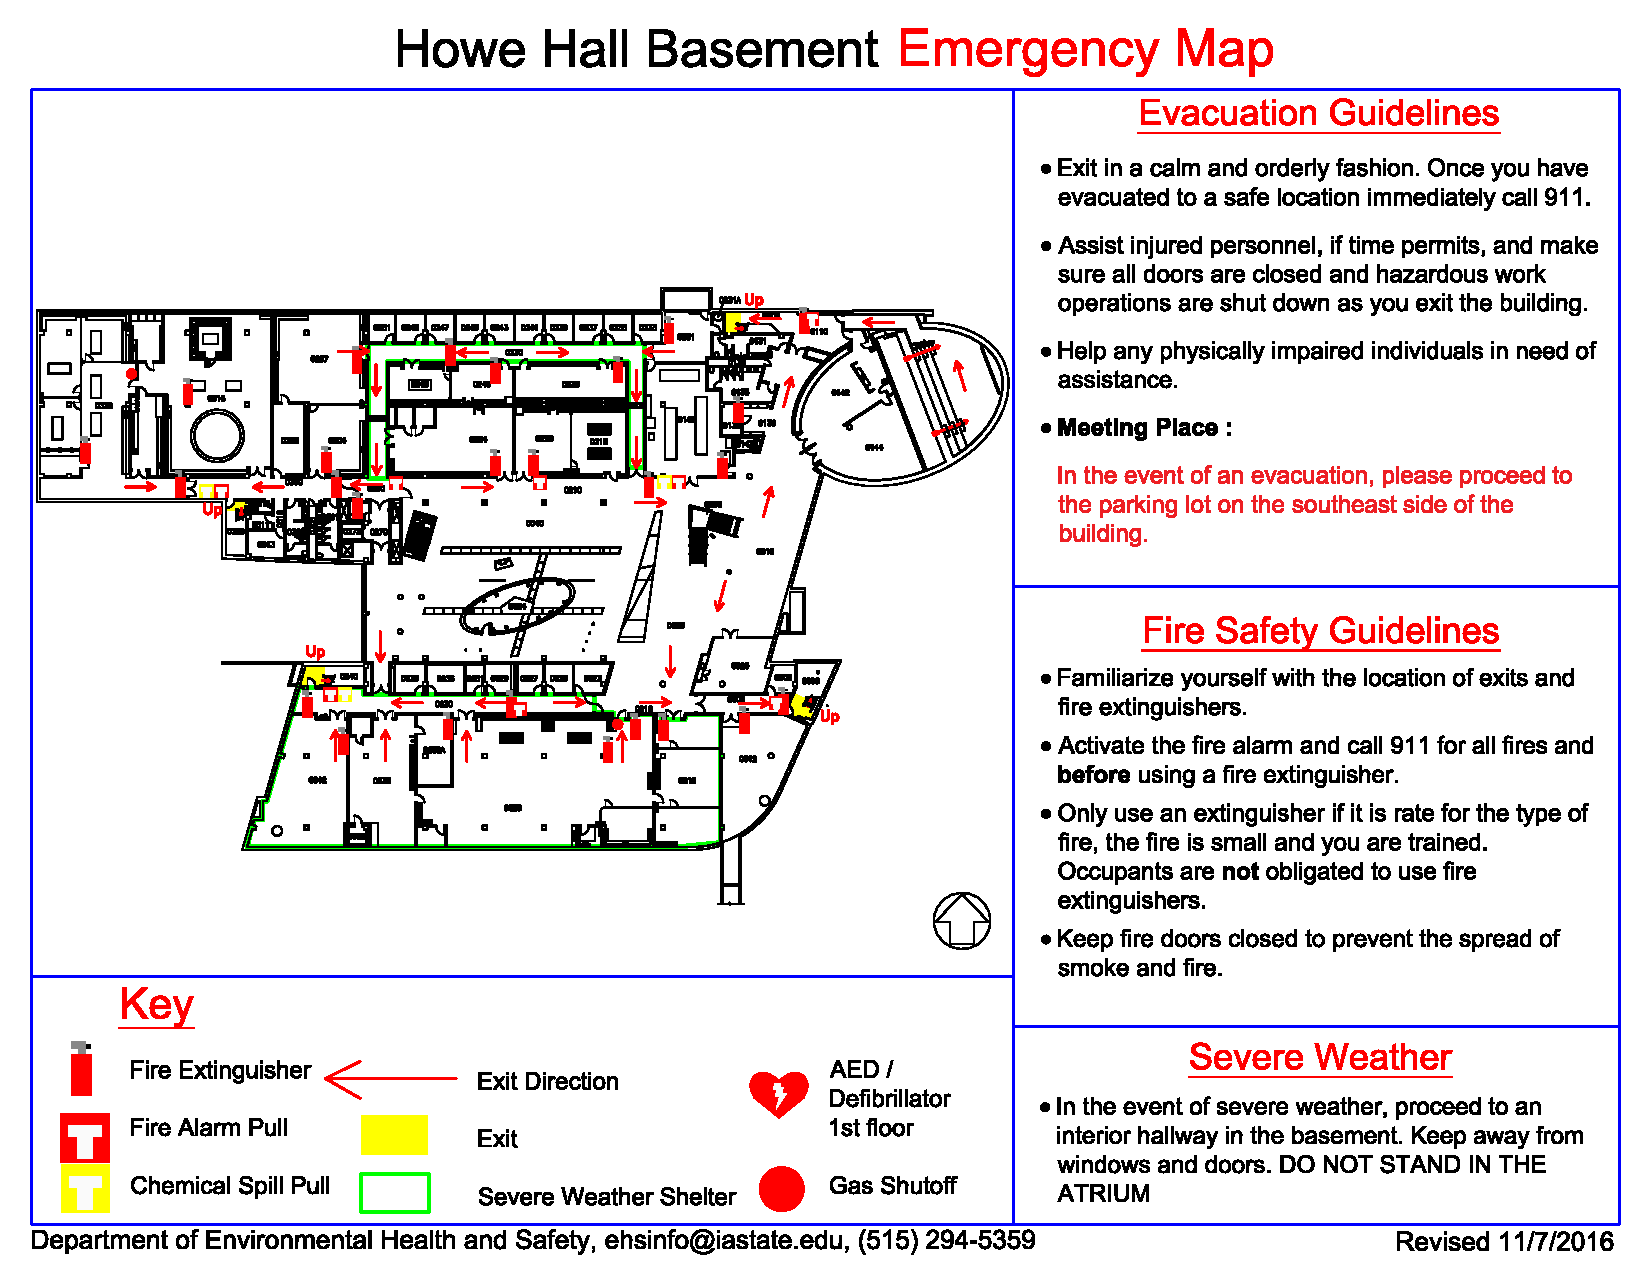
\includegraphics[width=6in]{Howe-Bsmt.pdf}
\caption{Howe Hall Evacuation Map}
\label{fig:Evac_map}
\end{figure}

The 0620 Lab Space is a designated tornado shelter and personnel may remain in the lab during severe weather.  In the event of a tornado all personnel should stay in the lab or in the most inner room of the lab.  Those spaces are 0620A, 0620B and 0620E within the lab space.

\chapter{Lab Facilities}
The lab has facilities that can be used by students for their projects.  This includes storage of their project materials, a conference room as well as additional storage for raw materials.  The lab also has work tables, work benches that projects can use for assembly and construction work on their projects.  Finally, the lab has several pieces of equipment that are used for design and construction such as a drill press, CNC machine, down draft table and computer lab.

\begin{figure}[ht]
\centering
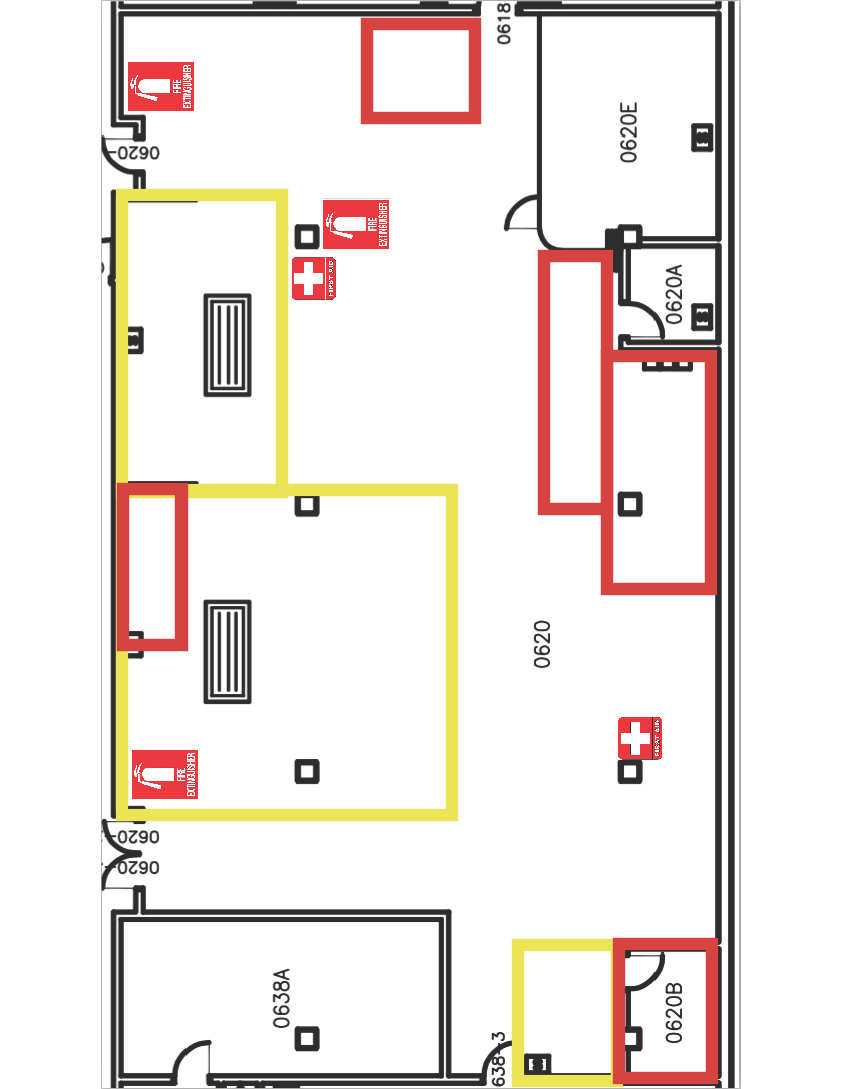
\includegraphics[width=5.8in]{images/0620_Floor_Plan.png}
\caption{0620 Floor plan with safety glasses (yellow), first aid, fire extinguishers, and restricted areas (red) marked}
\label{fig:0620_floor_plan}
\end{figure}

The M:2:I Lab has a fairly open concept and as such we have equipment that is often used that can generate hazards.  The lab has been organized to keep hazardous equipment in one area so that other areas may be used for less hazardous work.  Figure \ref{fig:0620_floor_plan} shows a floor plan of the lab with areas marked that are restricted or require safety glasses at all times.  Areas in yellow require safety glasses safety glasses at all times.  Areas in red are restricted to only M:2:I faculty, staff, lab monitors and lab technicians.  No students are permitted in these areas at any time.

\section{Project Storage Lockers}
The M:2:I Lab has storage lockers that projects can use to store their equipment, work in progress and finished parts.  The M:2:I Lab has full size lockers, smaller storage drawers and storage shelves to hold a variety of sizes of equipment and parts.  All M:2:I projects must be assigned these spaces.  If a project requires more space than what is currently available, they should talk to the M:2:I Program Coordinator.

\section{Storage Room}
The storage room is located in 0620B and contains building materials such as foam and wood. It also has spare parts from previous projects such as motors, servos, props and other smaller equipment.  Projects are free to use this material. In order to do so, groups must first seek out a lab monitor, who will open the room.  Lab monitors will keep track of the rough quantity that each group is using of each material. This will ensure that a groups are not using an excessive amount of materials. The storage room is for lab storage only; unauthorized objects will be jailed or requisitioned for lab supplies. Only under special circumstances will a group be allowed to store material in the storage room. This requires the approval of the M:2:I Program Coordinator.

If a project requires a large purchasing of materials and to have that stored, they must request the materials be ordered and must have permission of the M:2:I Program Coordinator to store items in the storage room.  Projects may have the items charged to their account.  This will be at the discretion of the M:2:I Program Coordinator.  

\section{Supply Room}
The supply room, located in 0620A, contains various cleaning materials and office supplies. This room is restricted to lab monitors and M:2:I faculty and staff only. If paper towels, markers, or any other related items run out, tell a lab monitor and they will take care of replacing the items in question. The supply room is strictly for lab use only and will not be used to store any project related materials.

\section{Conference Room}
The lab conference room is a space that has been set aside for use by M2I groups and for the Aerospace Engineering Department. Projects may request to use the conference room for project or team meetings.  In order to request using the conference room, you must email the M:2:I Program Coordinator.  A calendar will be kept near the Lab Monitors desk.

\section{Computer Lab Area}
The computer lab area houses 10 Dell computers running Windows 10 and a variety of software.  Software that is normally available to Engineering students such as Matlab, Solid Works, LabView, Microsoft Office, and others are installed on these machines.  In addition to these machines, the M:2:I Lab also has 24 Dell laptops that may be checked out for short durations.  

\section{3D Printing Area}
The 3D Printing Area is a restricted area that only authorized personnel are permitted in.  This area has the 5 3D printers that are used for both M:2:I and other projects.  If a M:2:I project wishes to print something on the 3D printers, they should contact the M:2:I Program Coordinator or Christine Nelson in 1200 Howe Hall.


\chapter{General Lab Procedures}
The following is basic procedures and guidelines that students should follow when performing certain actions in the lab.  These guidelines are meant as a starting point for students when working on their construction projects in the lab.  These are not meant to be a comprehensive guide, but should help students in getting started.  If you still have questions or concerns on a certain procedure, please visit with a lab monitor, lab technician or the M:2:I Program Coordinator.

\section{Sanding Procedures}
Sanding is a method in which we remove material from the object we are working with.  This is often needed in order to smooth the object, refine the shape, or even polish an object.

\begin{framed}
\begin{wrapfigure}{L}{0.14\linewidth}

\includegraphics[width=\linewidth]{images/important_icon.png}
\end{wrapfigure}
\ \\
Sanding will generate fine particulate matter that can be irritating to the skin eyes, or lungs.  Students sanding must wear eye protection and in most cases must wear a face mask to prevent this irritation.  Use of a downdraft table will also help minimize irritation.
\end{framed}
Sandpaper comes in many different grits. The higher the number of the grit, the finer the sandpaper. This lab has sandpaper that ranges from 60 grit to 1500 grit. When sanding, start at a lower grit number and step up one grit increment at a time until the desired surface finish is reached. 

All sandpaper is locked up in the tool crib and must be checked out by a lab monitor. It is up to you to understand what grit requirement you need and how to properly use sandpaper. The rest of this section will go over how to use sandpaper and grit numbers properly for different materials. If any questions remain, consult a lab monitor and they will recommend the correct grit and sanding procedure.

\subsection{Downdraft Table}
Groups that need to sand \emph{must} do so on the provided downdraft table. The M:2:I lab has one downdraft tables that groups may use for sanding or any activity that may produce small particulate.  To use the downdraft table, please follow the steps below.

\begin{enumerate}
\item Turn the power switch into the \textbf{ON} position. This is the left hand switch that is labeled \textit{Power}
\item Select the desired speed on the right hand switch labeled \textit{Speed}. The up position is \textbf{HIGH} and the down position is \textbf{LOW}
\item Sand on the top surface of the machine
\item If dust is not being pulled into the machine
\begin{enumerate}
\item Change the speed setting to \textbf{HIGH} if it is not already
\item If the speed is on \textbf{HIGH} and the dust is still not being collected, consult a lab monitor, the filter may be in need of replacement
\end{enumerate}
\item When finished sanding, sweep any remaining dust into the collection system prior to turning the power off
\item Turn the power switch into the \textbf{OFF} position
\item Clean up the immediate area
\end{enumerate}

If you have any questions about the downdraft tables or the tables are not working properly, see a lab monitor.  It also the responsibility of the user to clean up any material did not get pulled into the downdraft table.  Always clean up both on top of and around the downdraft table when finished.

\subsection{Wood}
Wood sanding procedure depends a lot on the type of wood being sanded. The most common used in the lab is oak, a hardwood, and balsa, a softwood.  The desired finish that the user wants also plays an important role, so it is important to know both the wood you are working with and what you want in the end.  Always make a plan on what you want to accomplish.  The following is some guidelines in making this plan.
\begin{enumerate}
\item Determine the type of wood that is going to be sanded
	\begin{enumerate}
	\item Hardwoods will require a lower starting grit whereas softwoods can use a finer grit to start with
	\item For most applications, starting with a 60 or 80 grit sandpaper is sufficient, for softwoods, using 100 grit to start with will also work.
	\end{enumerate}
\item Determine the type of finish required
	\begin{enumerate}
	\item If the wood needs to have a very fine finish, it will require more sanding and will require more steps between start and finish
	\item If the wood's finish is not entirely critical, only a few steps will be needed to achieve an acceptable finish
	\end{enumerate}
\item Start with an acceptable sanding grit and sand with the wood grain until the surface has a uniform look and feel
	\begin{enumerate}
	\item Use a piece of sandpaper until there is very little grit left on it or until the amount of material the sandpaper is removing is minimal, replace when the sandpaper is at this state
	\item When sanding with sandpaper, do not fold the sandpaper as this ruins the grit on one side, effectively wasting sandpaper
	\end{enumerate}
\item Depending on your requirements, step up to the next grit of sandpaper
	\begin{enumerate}
	\item Usually, if the starting grit was a 60, the next step up would be an 80. If its 80, the next step would be 100 and etc
	\end{enumerate}
\item Sand with each grit until the surface has achieved a smooth, uniform appearance before moving on to the next grit
\item Stop sanding when the surface has achieved an acceptable finish
\end{enumerate}

\subsection{Foam}
Sanding foam is quite different than sanding wood. Foam is much softer and does not require quite as low a starting grit and requires fewer steps from start to finish.  As with wood though, plan your actions to minimize wasting time and materials.
\begin{enumerate}
\item Generally 100 or 150 grit sandpaper is sufficient to sand foam and to get it to its desired shape.
\item Sand the foam until it reaches its desired shape
	\begin{enumerate}
	\item Since foam is much softer than wood, sanding will take much less time and require less effort
	\item Rarely will it be necessary to sand foam with sandpaper of a higher grit than 150
	\end{enumerate}
\item For most applications, one grit should be sufficient, however for finer finishes it may be necessary to use a second grit
\end{enumerate}

\subsection{Metal}
Unlike sanding both foam and wood, sanding metal removes very little material and is meant solely to provide surface finish. Sanding metal will require a great deal of time and effort. Metal also requires lower starting grits and more steps between start and finish than both wood and foam.
\begin{enumerate}
\item Determine current surface quality
	\begin{enumerate}
	\item It may be necessary to prepare the surface with a wire brush or grinder in order to remove surface obstructions and rust
	\end{enumerate}
\item Determine the finish that is necessary
	\begin{enumerate}
	\item Smooth surfaces require much less work than mirror like surfaces
	\end{enumerate}
\item Start with a relatively rough sandpaper to begin with. Generally a 60 grit should be sufficient
\item Sand until the surface has a uniform appearance
\item Step up to the next available grit and continue to sand until the surface scratches have been removed
\item Continue to sand and step up from grit to grit until the desired surface finish is reached
\begin{enumerate}
	\item To achieve a shiny, mirror-like surface, grits up to and in excess of 600 grit will likely be needed
\end{enumerate}
\end{enumerate}
\begin{framed}
\begin{wrapfigure}{L}{0.15\linewidth}

\includegraphics[width=\linewidth]{images/info_icon.png}
\end{wrapfigure}
\ \\
Iron metals have a thin layer called scale built up on the exterior of the metal. If a very shiny surface is desired, this layer will have to be completely removed. To do this a protective coating must be applied or the metal will oxidize.  This will undo all the work that was done to the part.  
\end{framed}
If you have further questions about working with metals, see the Program Coordinator or a lab monitor.

\section{Chemical Procedures}
Certain chemicals may also be used in the lab to achieve your final result in your construction.  These chemicals are often adhesives, etching, or painting.  As with any chemical, care must be taken when using these chemicals and all safety procedures must be observed.

\subsection{Adhesives}
Adhesives are frequently used in the Make to Innovate lab. When using adhesives, read all applicable labels and understand how the adhesive works. Seek a lab monitor's assistance if you are unsure as to how to use the adhesive correctly. Prior to using any adhesive, put down disposable paper or cardboard on the work surface being used to prevent spills or drips. Any spills or drips will be the responsibility of the student to clean up. Any subsequent damage resulting from improper use of adhesives will result in disciplinary actions.
\begin{framed}
\begin{wrapfigure}{L}{0.16\linewidth}
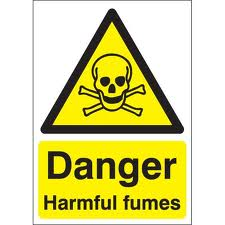
\includegraphics[width=\linewidth]{images/fumes_hazard.jpg}
\end{wrapfigure}
\ \\
Almost all adhesives produce fumes that can be harmful or toxic to humans.  Adhesives must be used in a well ventilated area.  Many of these fumes are also flammable, therefore they must be used away from any kind of ignition source.
\end{framed}
\subsection{Painting}
The Make to Innovate lab has brush-on paint available for use by groups. Painting can be done in the lab on the workbenches with lab monitor approval. All painting must be done on cardboard or paper to prevent spills. All spills must be cleaned up by groups immediately. Projects must have travelers affixed to their project if the project is to be left out to dry. 

Spray paints are prohibited in the lab. Make to Innovate will not supply spray paints, and groups are not allowed to bring in their own spray paints.  If spray paining must be used, permission must be obtained from the M:2:I Program Coordinator.  Spray painting is only permitted outside of Howe hall with proper PPE used and proper protection of the grass or concrete surface.  
\begin{framed}
\begin{wrapfigure}{L}{0.16\linewidth}
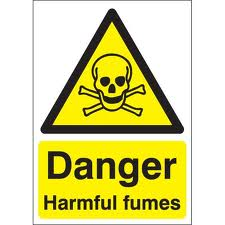
\includegraphics[width=\linewidth]{images/fumes_hazard.jpg}
\end{wrapfigure}
\ \\
Almost all paints produce fumes that can be harmful or toxic to humans.  Paints must be used in a well ventilated area.  Many of these fumes are also flammable, therefore they must be used away from any kind of ignition source.
\end{framed}
% Basic Electronics Training
% Updated 1/24/2017

\chapter{Basic Electronics Training} \label{basic_electronics}
\section{Introduction}
The M:2:I lab has equipment that is suitable for a wide range of electrical work, diagnostic and repair.  The lab has a sectioned off area that is dust controlled and has work surfaces that is static controlled.  This creates a suitable work environment for working on a number of electrical projects.

The electrical area has work benches that is divided up to 3 stations.  Station 1 contains advanced diagnostic and soldering equipment and requires additional training beyond the scope of this section.  Station 2 and 3 has basic diagnostic soldering equipment and will be covered in this section.

Station 2 and 3 has the following equipment at each station.  In addition, these stations are suitable for the following activities.

\begin{itemize}
\item Soldering and de-soldering components
\begin{enumerate}
\item Through hole components
\item Surface mount components
\end{enumerate}
\item Lab bench power supply
\begin{itemize}
\item 0 - 30 VDC @ 3 amp controlled supply
\item power consumption logging
\end{itemize}
\item Waveform generation
\item Waveform measurement
\end{itemize}

It should be noted that the work bench is a Electro Static Discharge (ESD) safe and is designed to minimize ESD when used properly.  This requires that users are properly grounding themselves and using the wrist-straps that are attached to the bench.  An additional work mat is also at each station which is also ESD safe and helps protect the bench from soldering.

\begin{framed}
\begin{wrapfigure}{L}{0.14\linewidth}

\includegraphics[width=\linewidth]{images/important_icon.png}
\end{wrapfigure}
\ \\
Students working at the electronics stations must take care to not damage any of the mats.  No cutting is permitted at any time with these mats and care should be taken when soldering to prevent burning.
\end{framed}

\section{Hazards}
The following are possible hazards when working with any of the equipment in the electrical work bench area.  Please take note of these hazards and make sure you understand the possible dangers and the steps needed to reduce possible harm to yourself.

\begin{framed}
\begin{wrapfigure}{L}{0.15\linewidth}
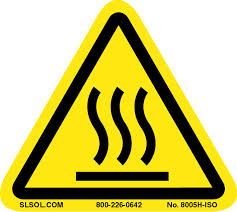
\includegraphics[width=\linewidth]{images/burn_hazard.jpg}
\end{wrapfigure}
\ \\
Burns are possible both from the soldering iron and heated materials during the soldering process. Always utilize the soldering iron stand and always look when reaching for the iron. Never solder with unsupported materials or over your body. Heated materials may fall from the connection and cause severe burns.
\end{framed}

\begin{framed}
\begin{wrapfigure}{L}{0.15\linewidth}

\includegraphics[width=\linewidth]{images/electrocution_hazard.jpg}
\end{wrapfigure}
\ \\
Electrocution is always a possibility when working with electronics. Keep liquids away from the workbench at all times. Always double check your electrical connections. Only energize the circuit when necessary and move the circuit as little as possible while energized. Proper use of the over-voltage and over-current controls can help to minimize any damage or injury caused by a short circuit condition.
\end{framed}
\ \\
\ \\
\begin{framed}
\begin{wrapfigure}{L}{0.16\linewidth}
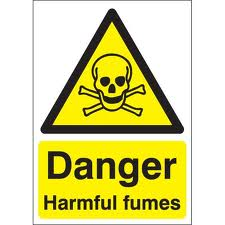
\includegraphics[width=\linewidth]{images/fumes_hazard.jpg}
\end{wrapfigure}
\ \\
Hazardous fumes may result from the decomposition of solder, fluxes, cleaning agents and other soldering substances or from substances on the materials being soldered. Fumes released during soldering are generally within allowed exposure limits but care should be taken.  Proper use of the smoke extractor will minimize any possible effects from these fumes.
\end{framed}

\subsection{Chemicals}
Chemicals used while soldering, including lead, may cause skin or eye irritation or may be ingested. Gloves should be worn when dealing with any substance marked as hazardous and hands should always be washed after soldering or handling soldering materials.

\section{Electronics Equipment}
The following is additional information on each piece of equipment that you can find at both station 2 and 3.  Information on Station 1 can be found in the Advanced Training in Chapter 

\subsection{Weller WES51 Soldering Iron}
The Weller WES51 shown in Figure \ref{fig:wes51} is a standard soldering iron that has the following features:

\begin{itemize}
\item 50 watt pencil iron,
\item Replaceable tip sizes,
\item 350 to 850 degrees F,
\item Temperature stability +/- 10 degrees F,
\item Temperature accuracy +/- 10 degrees F.
\end{itemize}

\begin{figure}[ht]
\centering
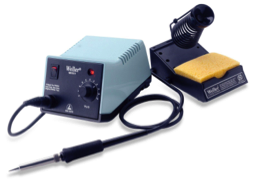
\includegraphics[width=2in]{images/wes51.png}
\caption{The Weller WES51 Soldering Iron}
\label{fig:wes51}
\end{figure}

The WES51 has the ability to have both different sizes and shapes of tips that can be used.  In general, the soldering iron is equipped with a fine conical tip.  This type of tip is suitable for light general purpose soldering and for some surface mount soldering.  The lab does have some some other sizes and shapes of tips available.  Please see a lab monitor or Matthew Nelson if you need a different tip.

\subsection{Rigol DP832 Programmable DC Power Supply}

The Rigol DP832 shown in Figure \ref{fig:dp832} is a programmable lab bench DC power supply.  It has the following features:

\begin{itemize}
\item Three adjustable outputs: 30V/3A, 30V/3A, 5V/3A,
\item Up to 195W total power,
\item Programmable over-voltage/over-current protection,
\item Programmable voltage waveform,
\item Voltage/Current/Power waveform display/logging.
\end{itemize}

\begin{figure}[ht]
\centering
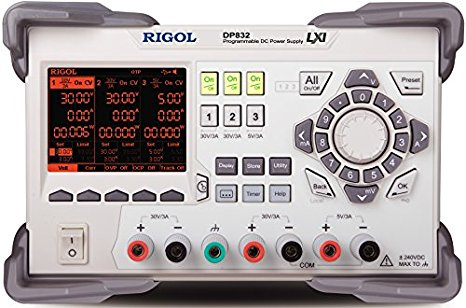
\includegraphics[width=2in]{images/dp832.jpg}
\caption{The Rigol DP832 DC Power Supply}
\label{fig:dp832}
\end{figure}

\subsection{Rigol DS1102E Digital Oscilloscope}
The Rigol DS1102E Digital Oscilloscope shown in Figure \ref{fig:ds1102e} is suitable for reading a number of waveforms for diagnostic purposes.  It has the following features:

\begin{itemize}
\item Two channel, 1 GSa/s maximum real-time sample rate,
\item 100 MHz bandwidth,
\item 10 Kpts memory depth,
\item Image and data export to USB drive.
\end{itemize}

\begin{figure}[ht]
\centering
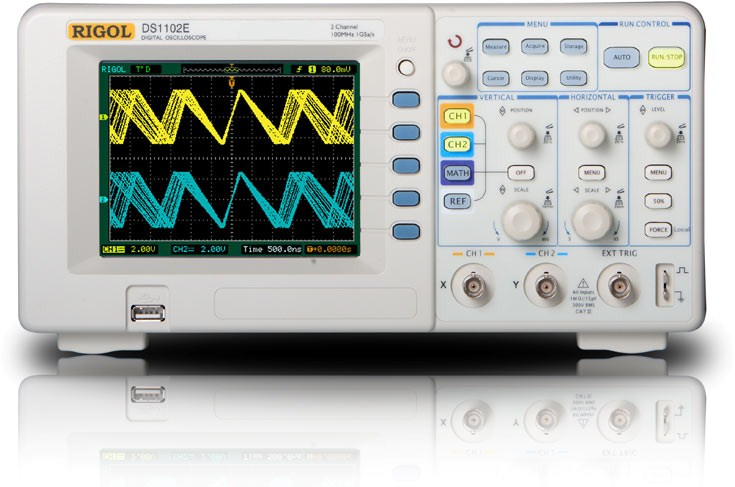
\includegraphics[width=2in]{images/DS1102E.jpg}
\caption{The Rigol DS1102E Digital Oscilloscope}
\label{fig:ds1102e}
\end{figure}

\subsection{Rigol DG1022A Arbitrary Waveform Generator}
The Rigol DG1022A shown in Figure \ref{fig:dg1022a} is a lab bench wave form generator that is able to generate a number of waveforms and frequencies for testing and diagnostics.  This generator has the following features:
\begin{itemize}
\item Two channel arbitrary waveform up to 25 MHz,
\item Modulation functions (AM, FM, PM, FSK, etc),
\item Frequency counter up to 200 MHz,
\item 100 MSa/s sample rate, 14 bit accuracy.
\end{itemize}

\begin{figure}[ht]
\centering
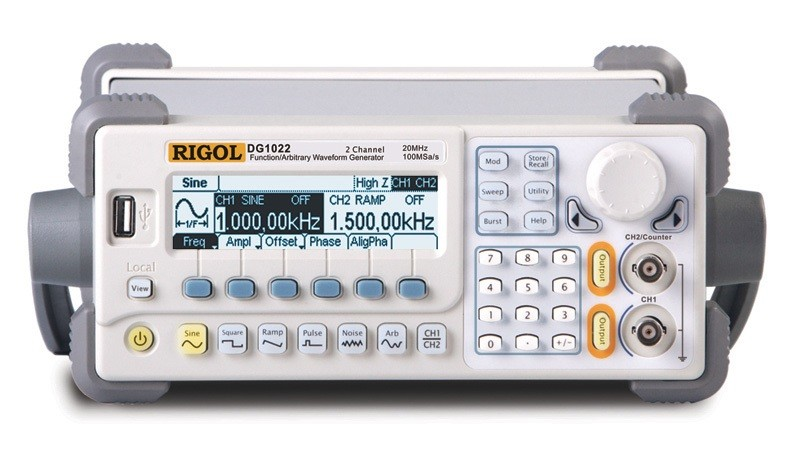
\includegraphics[width=2in]{images/dg1022a.jpg}
\caption{The Rigal DG1022A Waveform Generator}
\label{fig:dg1022a}
\end{figure}

\chapter{Electronics Procedures}
Student should be familiar with the general procedures for using the equipment at the electronics bench before using them.  The following procedures are there to provide guidance to students in using the equipment at the electronics workbench.  It is not a comprehensive guide but should help students in getting started with the equipment.  If at any time you have questions please see the M:2:I Program Coordinator.

\section{Soldering Procedures}
Soldering is a skill that does take some practice.  A good solder joint will provide both a good electrical connection and securely hold contact or pin to the printed circuit board.  A poor solder connection however can cause intermittent behavior in the circuit and can cause the circuit to fail.

The electronics lab has two types of solder, lead based and lead-free solder.  Lead-free solder is recommended for most projects, but in some cases, such as critical applications, it should not be used.  An interesting fact, the lead-free solder (Tin-Silver-Copper) was actually developed here at Iowa State University in the Ames Laboratory and with Sandia National Labs-Albuquerque.

\begin{framed}
\begin{wrapfigure}{L}{0.14\linewidth}

\includegraphics[width=\linewidth]{images/important_icon.png}
\end{wrapfigure}
\ \\
The use of leaded solder can be hazardous to the students health.  If leaded solder must be used, it should be handled with gloves and soldering should take place with a fume extractor in use.  Doing this will minimize the introduction of lead into the body which is toxic.
\end{framed}

\subsection{Soldering}

\begin{framed}
\begin{wrapfigure}{L}{0.15\textwidth}
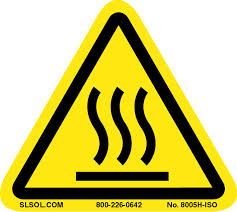
\includegraphics[width=.7in]{images/burn_hazard}
\end{wrapfigure}
\ \\
The tip on a soldering can reach temperatures of 400 C (750 F) and higher.  Always use caution when using a soldering iron and always be aware of both your surroundings and where the soldering iron is.  While most surfaces in the electronics area can handle short durations of heat, you can not.
\end{framed}

\begin{framed}
\begin{wrapfigure}{L}{0.15\textwidth}
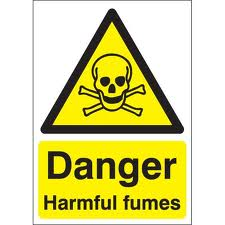
\includegraphics[width=.7in]{images/fumes_hazard}
\end{wrapfigure}
\ \\
Fumes produced from soldering can be hazardous to your health with both leaded and lead free solder.  Fumes can irritate and cause harm to both your lungs and eyes.  You should always use one of the ventilation fans to pull the fumes away from you.
\end{framed}
Soldering involves heating up the \emph{pad} and the \emph{pin} to allow the solder to flow and on the part.  In most cases you \emph{do not} want to heat up the part itself.  In many cases doing so will result in damage to the part.  The key to soldering is apply even heat to the pad and allowing the solder to flow on the pad and pin.  A good solder joint will look like Figure \ref{fig:good_solder}.  The following steps should be followed to ensure good soldering techniques.

\begin{enumerate}
\item Ensure station has a brass sponge or a wetted sponge.
\item Set the iron to the correct temperature, when the LED is rapidly flashing the iron is at the set temperature
\item Clean the iron using the brass sponge or wet sponge
\item Tin the tip of the soldering iron
\item Heat the pad or joint and then apply solder to the pad or joint
\item Once the solder is melting apply enough to ensure a good connection
\item Remove the iron once done with the solder
\item Clean the tip as needed to remove excess solder
\item When done, clean the iron, return it to its holder and turn off the iron

\end{enumerate}

When cooling, take care to make sure the pin or part does not move.  If it does, this might create a cold solder joint which may cause intermittent behavior.  If you think the part did shift, you can often fix this by re-flowing the solder and allowing it to cool again.

\begin{figure}[ht]
\centering
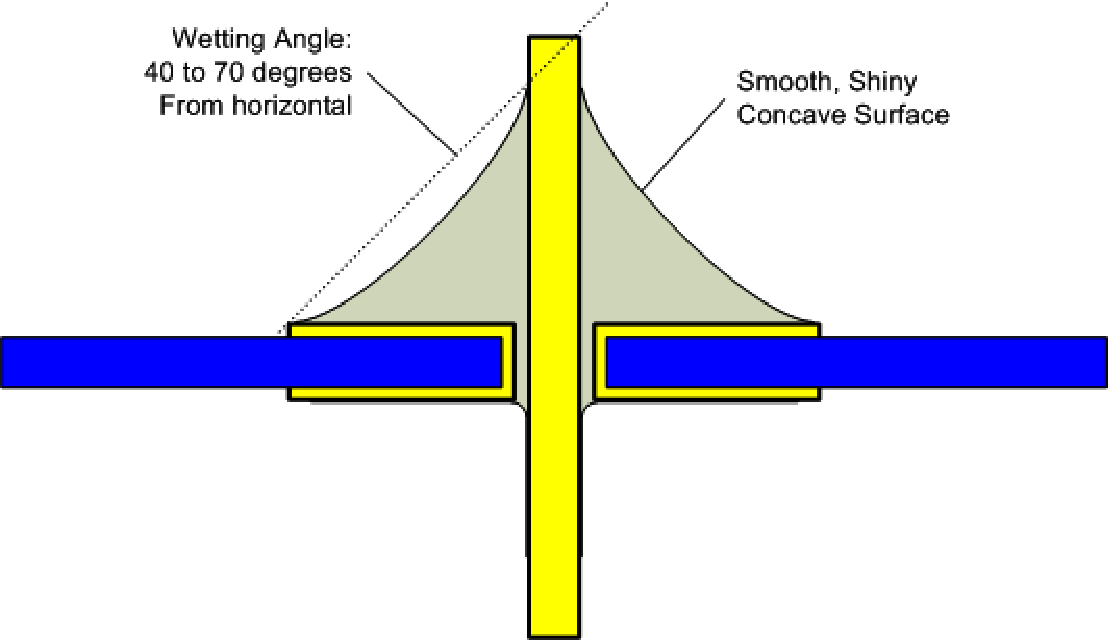
\includegraphics[width=4.5in]{images/tools_Solder_Joint.pdf}
\caption{A good solder joint. (Source: Adafruit.com)}
\label{fig:good_solder}
\end{figure}

\subsection{Tips and Tricks}
For the temperature, the iron should be set to between 343 - 371 C (650 - 700 F) for lead based solder and 371 - 400 C (700 - 750 F) for lead free solder.  Through hole and larger components will require temperatures in the upper area of these ranges while smaller components and surface mount can often use cooler temperatures.  When soldering, the solder will cool quickly and should cool to a shiny almost mirror finish.  A dull finish may indicate a poor solder connection.

When cleaning the iron, you should always have a thin coat of solder on the iron.  The point of cleaning is not to remove the solder, it is to keep the tip tinned.  Excess solder should removed when needed and when done soldering.

If the solder does not flow, the iron may be too hot and burning the tin/flux too quickly. If reducing the iron temperature does not help, you may need to use additional flux. You may also need to replace the tip or there could be a problem with the iron.  Contact a lab monitor or contact Matthew Nelson if you have any other questions or concerns with soldering.

\section{Power Supply}\label{power_supply}
The power supply is used to provide a regulated power source to a circuit under test. The power supply can also measure and record the power consumed by the circuit.

\begin{framed}
\begin{wrapfigure}{L}{0.15\textwidth}

\includegraphics[width=.7in]{images/electrocution_hazard}
\end{wrapfigure}
\ \\
Both the power supplies used and your circuit may cause electrocution.  No food or drink is allowed in the electronics area and keep water usage for the sponges to a minimum.  Only energize your circuit when ready and use the over-voltage and over-current features on the power supply.
\end{framed}
\subsection{Basic Operation}
\begin{enumerate}
\item Select an appropriate channel by pushing the corresponding channel select button and wiring your circuit to the corresponding output terminals
\item Press the Voltage soft-key and program the desired output voltage using the numeric keys or the dial
\item Press the Current soft-key and program the desired output current using the numeric keys or the dial
\item Press the OVP and/or OCP soft-keys to set the desired over-voltage or over-current protection values and again to enable the protection mode
\item Turn the channel on or off by pressing the corresponding On/Off button 
\end{enumerate}

When the load voltage is higher than the programmed value, the power supply will operate in constant voltage mode and limit to the programmed voltage.  When the load current is higher than the programmed value, the power supply will operate in constant current mode and limit to the programmed current.  If the load current or voltage crosses an enabled threshold, that channel will shut down.
\subsection{Timer Operation}
Timer operation allows the user to program voltage and current steps and associated time intervals.  This may be useful for testing a range of voltages and/or current values.  To use this feature, follow these steps.

\begin{enumerate}
\item Press the Timer button to display the timer interface.
\item Press the Timer Set soft-key to set the timer parameters.
\item After setting the timer parameters, press the Timer button and then the Timer softkey to enable the timer.
\end{enumerate}

\section{Oscilloscope}
\subsection{Basic Operation}
\begin{enumerate}
\item Compensate the probe for each channel you will be using (Optional)
\begin{enumerate}
\item Set the switch on the probe to 10X.
\item Press the channel button corresponding to the channel you are using and set the attenuation factor to 10X.
\item Attach the probe lead to the compensation connector and the ground lead to the ground connector.
\item Press the Auto button and wait a few seconds.
\item A square wave will be displayed on the screen, adjust the compensation trimmer on the probe until the waveform edges are square.
\end{enumerate}
\item Attach the probe to the circuit under test.
\item Press the Auto button or adjust the vertical and horizontal div controls as desired.
\end{enumerate}
For most measurements, the probe should be left in 10X mode for the best results.

\subsection{Adjusting the Display}

\textbf{Vertical}
The vertical scale of a channel can be adjusted by pressing the channel button of interest (CH1 or CH2) and then turning the scale knob. You can switch between coarse and fine adjustment by pressing the scale knob. The current scale is displayed on the bottom line of the display. To change the vertical position on the display, turn the position knob. While adjusting the position control, a voltage is displayed, indicating the voltage offset from the ground reference. You can instantly return the offset to zero by pressing the position knob.

\textbf{Horizontal}
The horizontal time scale can be adjusted by turning the horizontal scale knob. You can move the displayed waveform left and right by turning the horizontal position knob. Pressing the position knob will instantly center the waveform. Pressing the scale knob will enable zoom mode which will allow you to inspect the waveform in greater detail.
\subsection{Performing Measurements}
\textbf{Automatic}
\begin{enumerate}
\item Press the Measure button.
\item Use the Source soft-key to select which channel the measurement is performed on.
\item Press the Voltage or Time soft-key to select the type of measurement or the Clear softkey to clear any on screen measurements.
\item Press the soft-key corresponding to the specific measurement you wish to perform. The result will be displayed on screen.
\end{enumerate}
\textbf{Cursor}
Cursor based measurements can be used to manually measure time or amplitude parameters that cannot be performed automatically.  Follow these steps to use the cursor.
\begin{enumerate}
\item Press the Cursor button.
\item Use the Mode soft-key to select the manual mode.
\item Use the Source soft-key to select which channel the measurement is performed on.
\item Use the Type soft-key to select X or Y measurements.
\item Use the A and B soft-keys and the multi-function knob to move the cursors and see the results on screen.
\end{enumerate}
\section{Waveform Generator}
\subsection{Basic Operation}
The following steps will get you started in the basics of using the waveform generator.
\begin{enumerate}
\item Press the CH1/CH2 button to select the channel of interest.
\item Press the button corresponding to the type of waveform you would like to generate.
\item Press the Freq soft-key and enter the desired frequency using the dial or number pad.
\item Press the Ampl soft-key and enter the desired amplitude using the dial or the number pad. By pressing the Ampl key a second time, you may enter the desired maximum signal level (HiLev).
\item Press the Offset soft-key and enter the desired DC offset using the dial or the number pad. By pressing the Offset key a second time, you may enter the desired minimum signal level (LoLev).
\end{enumerate}
Double check the parameters you have entered before enabling the channel output. Press the View button to change the display to a view that allows you to check the frequency and amplitude at the same time. Then press the Output button next to the channel that you are using to enable the output.

\chapter{Foam Working Training} \label{foam_training}

\section{Introduction}

This training will cover the basics about how to create a project out of foam. Best practices on how to properly use adhesives, cut and shape foam, and coat foam will be covered to ensure an adequate knowledge of foam working.
\section{Hazards}

The following is possible hazards when working with foam and any of the equipment used on the foam.  Please take note of these hazards and make sure you understand the possible dangers and the steps needed to reduce possible harm to yourself.

\begin{framed}
\begin{wrapfigure}{L}{0.15\linewidth}
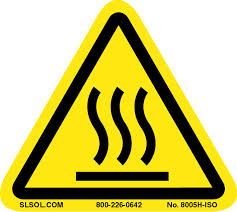
\includegraphics[width=\linewidth]{images/burn_hazard.jpg}
\end{wrapfigure}
\ \\
Several tools used to shape and cut foam use heat to melt the foam. In order to reduce burn risk, keep appendages away from the heat source and handle hot tools and materials with care. Always be familiar with safety and operating procedures of the tool being used in order to minimize burn risks. Always be aware of your surroundings and others while working with hot tools and materials.
\end{framed}
\ \\
\begin{framed}
\begin{wrapfigure}{L}{0.15\linewidth}

\includegraphics[width=\linewidth]{images/electrocution_hazard.jpg}
\end{wrapfigure}
\ \\
Some of the tools used while shaping foam require power to operate. These tools can result in electrocution if used improperly. Always check cords on plugged in equipment for damage prior to use. Do not use a piece of equipment that has a damaged or frayed cord. Report any damage to a lab monitor immediately. Always ensure that when plugging in equipment, the plug is fully inserted into the outlet and has a snug fit. Cords that are not securely plugged in present a potential electrocution hazard.
\end{framed}

\begin{framed}
\begin{wrapfigure}{L}{0.16\linewidth}
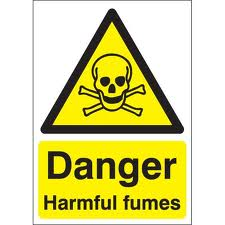
\includegraphics[width=\linewidth]{images/fumes_hazard.jpg}
\end{wrapfigure}
\ \\
Shaping foam can result in fumes. These fumes are not dangerous in the quantities seen while cutting foam correctly. In order to reduce any possible adverse effects, however, use a ventilation system when possible. Avoid excessive heat while cutting foam as the higher the temperature, the higher the quantity of fumes created. If nausea or light-headedness occur as a result of foam fumes, report it to a lab monitor and they will help you get to fresh air.
\end{framed}

\begin{framed}
\begin{wrapfigure}{L}{0.15\linewidth}

\includegraphics[width=\linewidth]{images/cut_hazard.jpg}
\end{wrapfigure}
\ \\
Hobby knives and other such tools used to shape foam have the potential to cause injury if used carelessly or improperly. Having the appropriate training that each tool requires is the best way to minimize the risk of cuts. Always make sure that your immediate surroundings are cleared of potential hazards and other people before using cutting tools as this helps reduce the risk of injury to both yourself and others. Always cut away from yourself and bystanders. Do not wear loose fitting clothing as this can be caught in the cutting tool and cause injury.  
\end{framed}

\subsection{Chemicals}
Chemicals have the potential to cause injury from mild skin and eye irritation to severe burns and potentially death. In order to minimize this risk, be familiar with the chemical prior to use. Read and follow all safety information listed on the chemical. Always use a proper vent hood when dealing with chemicals that create harmful fumes.

\section{Foam Safe Adhesives}
There are many different adhesives which can be used with foam.  Some work well, others do not. Many types of adhesives can produce toxic fumes and must be handled with care.  Always consult with a lab monitor before using an adhesive that you are not familiar with.
\subsection{Epoxy}
Epoxy is acceptable for almost any foam gluing application.  It is available in fast and slow curing times.  Epoxy is a high strength resin based adhesive, and can act as a structural glue.  Epoxy should be used for most foam constructions.  However, it is not very sandable.
\subsection{Foam Safe CA}
Foam safe CA (cyanoacrylate), as the name implies, is a super glue that is safe for foam.  It comes in several different viscosities, and is sometimes referred to as “odorless” CA.  CA accelerator can be sprayed on the adhesive for instant curing.  Foam safe CA works well for joining foam surfaces, and is not sandable
\subsection{Foam Fusion}
Foam Fusion is a type of adhesive for EPS foam.  It has a long cure time, but is sandable and hotwire safe.  In house tests have shown this adhesive to be stronger than the foam itself.
\subsection{Hot Glue}
Hot glue, which can be used on several types of foam, is not recommended for construction.  It is very low strength, and does not soak into the foam, creating a very weak joint.  Hot glue can also melt into the foam, for some types of foam, if hot glue must be used, a low temp glue should be used with the appropriate gun set to low temperature.  Hot glue is also not sandable, and will cause valleys to be formed around the joint if attempted.  Again, hot glue is not a structural adhesive, and therefore should not be used on high stress joints, such as wing spars, wing saddles, wing butt joints, and empennage attachments on aircraft.  Consult a lab monitor for advice on proper glue joint practices and applications.
\section{Cutting/Shaping Foam}
Cutting and shaping foam can be done in a variety of different ways. The most common are using a hot wire cutter, using a hot knife, or using a hobby knife.  The M:2:I Lab has hot wire and hot knife cutters that can be used for this purpose.  The following goes into instructions on using these tools with foam.

\chapter{Hot wire Cutters}
A hot wire cutter utilizes a heated wire to precisely melt foam. This is accomplished by running electricity through a relatively thin wire. As the current passes through the wire, the wire heats up. Most hot wire cutters have a unit that regulates the current passing through the wire in order to adjust the heat that the wire is producing. There are several types of hot wire cutters that this lab uses.

\section{Vertical Hot Wire Cutting Station}
\begin{framed}
\begin{wrapfigure}{L}{0.15\textwidth}
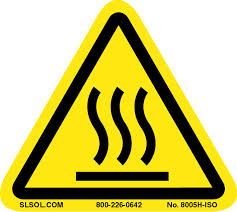
\includegraphics[width=.7in]{images/burn_hazard}
\end{wrapfigure}
\ \\
The wire on the foam cutter can reach high temperatures that can cause severe burns.  Care should be taken at all times when using the vertical cutter to avoid possible burns.
\end{framed}

\begin{framed}
\begin{wrapfigure}{L}{0.15\textwidth}
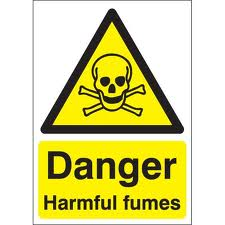
\includegraphics[width=.7in]{images/fumes_hazard}
\end{wrapfigure}
\ \\
Depending on the foam and if any hot wire safe adhesive is used fumes may be generated from using the hot wire cutter.  Make sure any adhesive you use is safe for hot wire cutting and minimize exposure to any fumes generated during cutting.
\end{framed}

The vertical hot wire station shown in Figure \ref{fig:verthotwire} uses a vertical wire that is set perpendicular to the work surface to cut out shapes from foam. This station ensures that the cut has as little taper to the cut as possible. In addition, the table also has slots set up for a mobile fence to ensure that straight cuts can be made from virtually any angle.

\begin{figure}[ht]
\centering
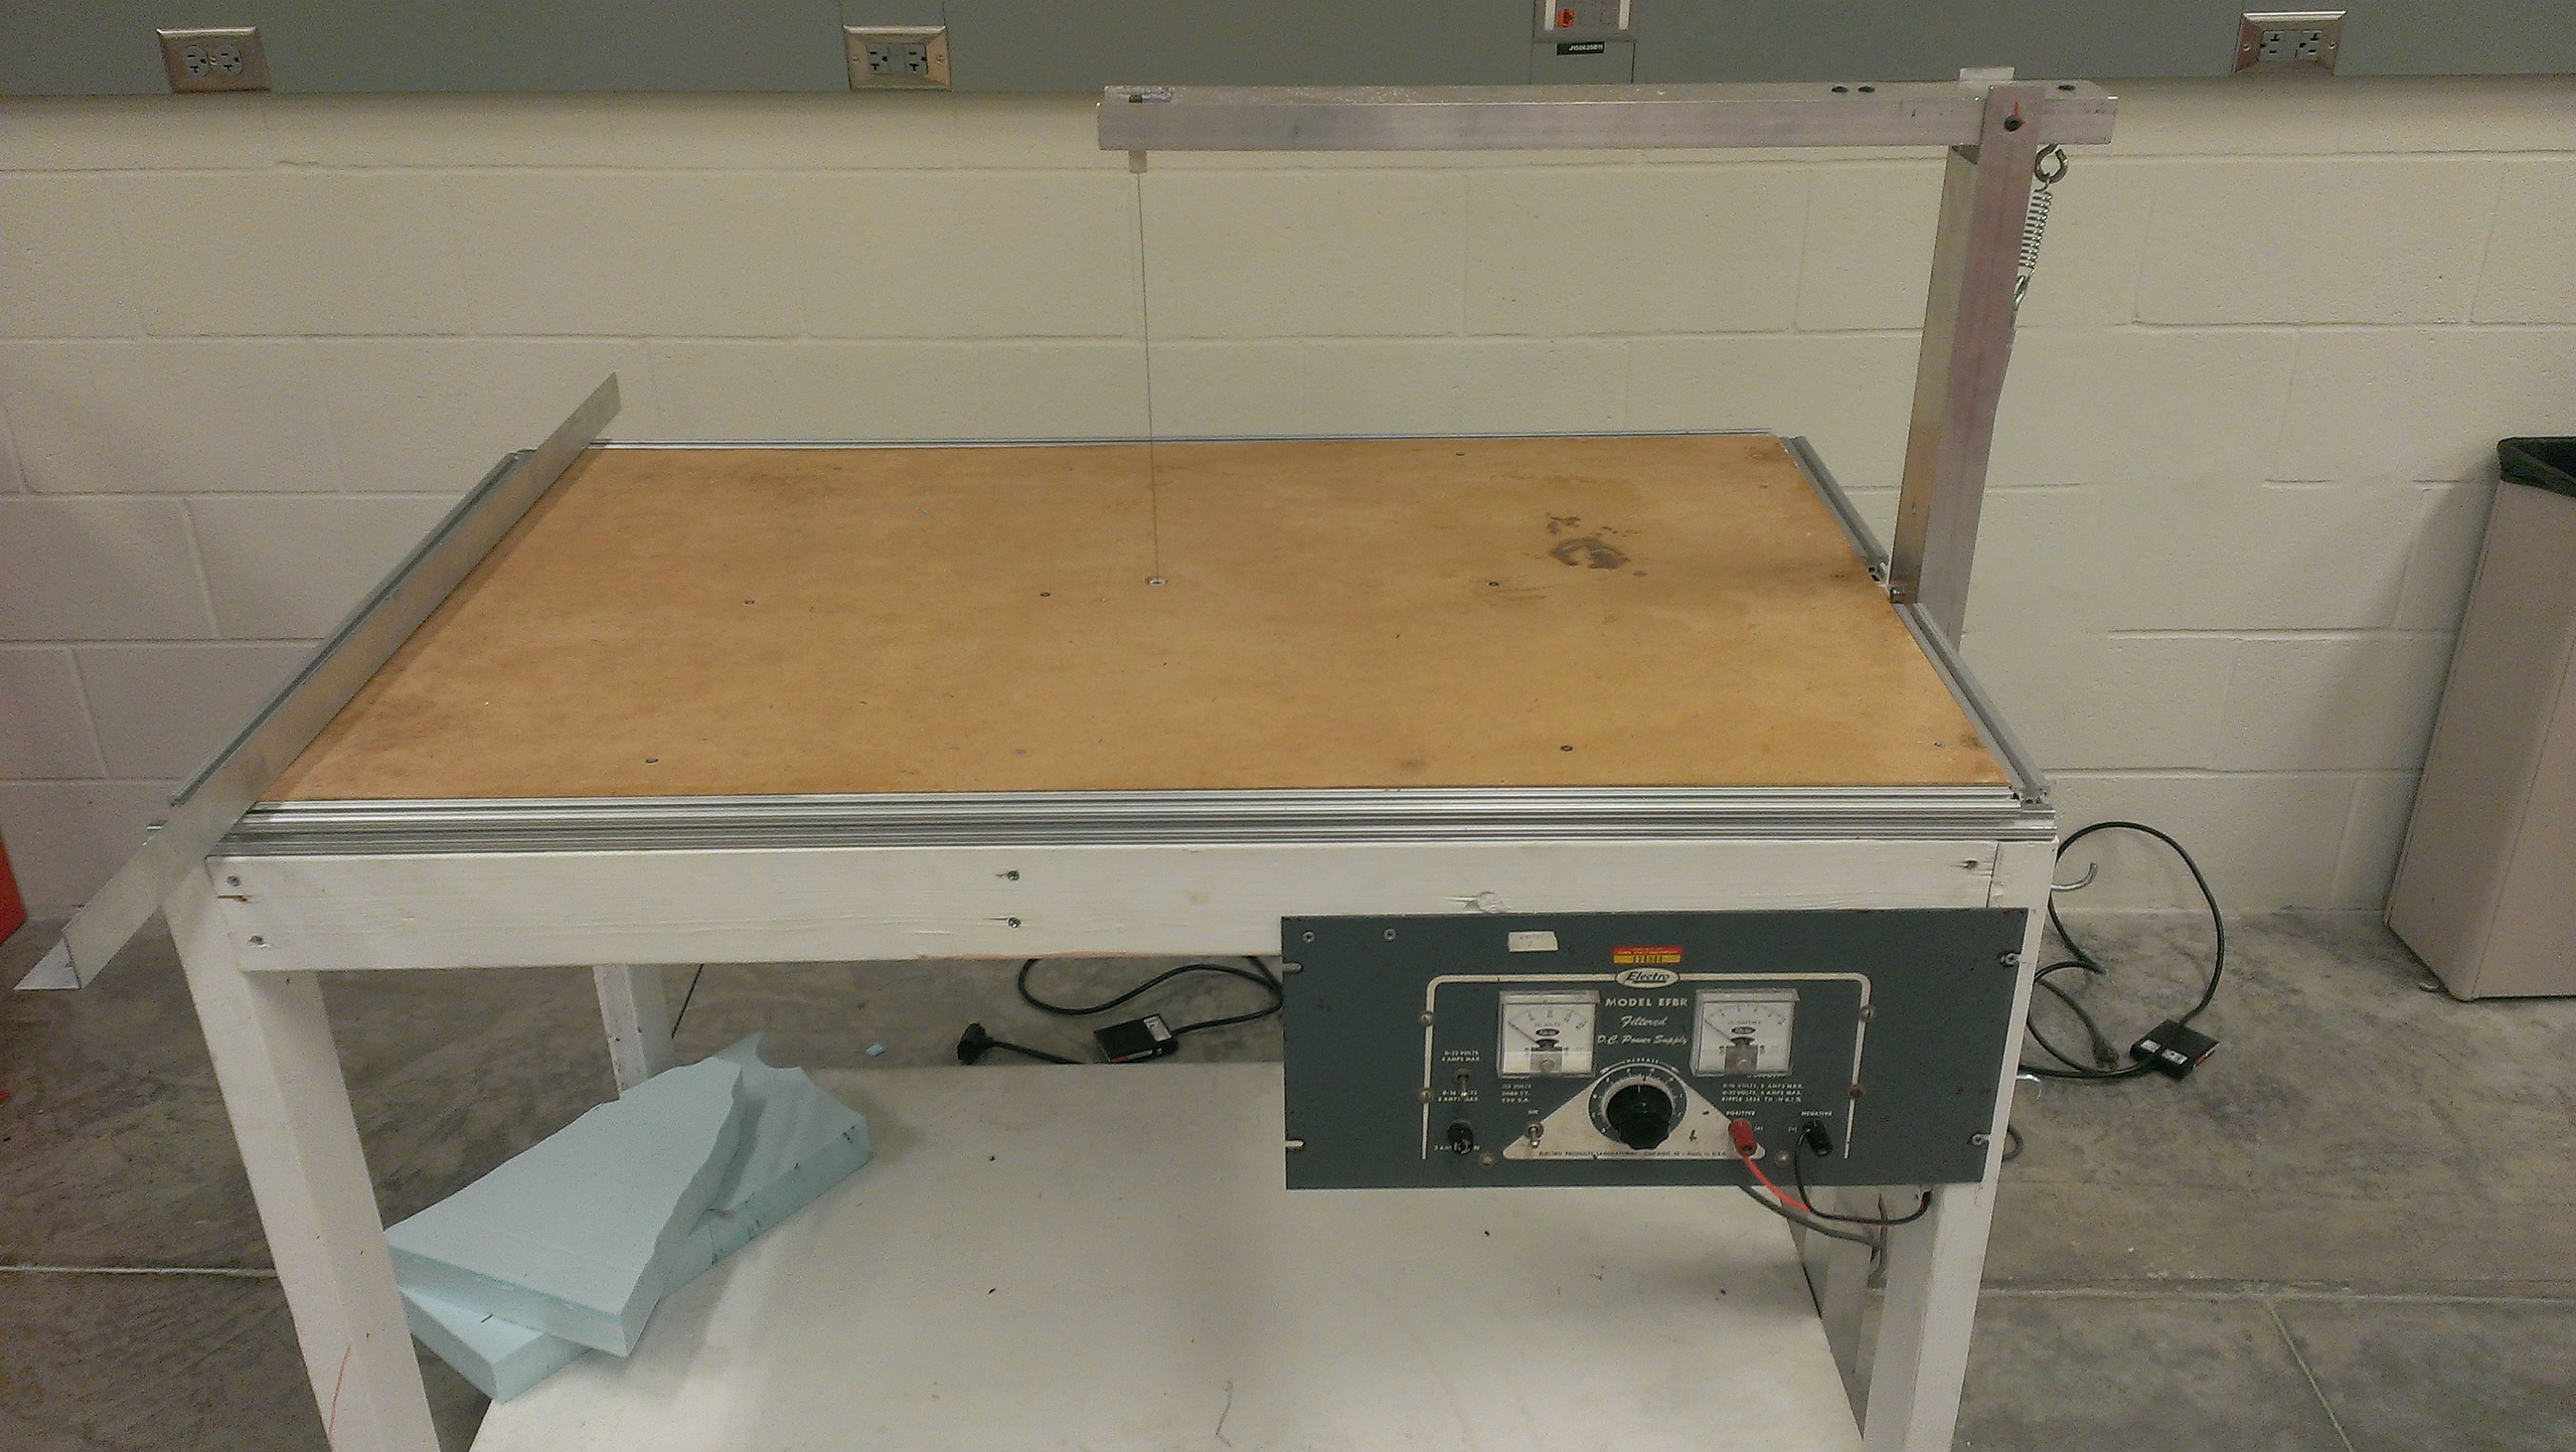
\includegraphics[width=4in]{images/IMAG0198}
\caption{Vertical Hot Wire Cutting Station}
\label{fig:verthotwire}
\end{figure}

\subsection{Operation}
To use the vertical hot wire cutting station, follow these instructions.

%\begin{figure}[h]
%\centering
%\includegraphics[width=2in]{../images/IMAG0222}
%\caption{Power and Heat settings on the power supply}
%\label{fig:hotwirepower}
%\end{figure}
\begin{enumerate}
\item Turn the Power setting to ON
\item Set the Heat Setting to the appropriate level
\begin{enumerate}
\item Turn clockwise to increase the heat output
\item Start on the lowest setting and slowly increase until the wire starts cutting smoothly
\item The correct heat setting will partially depend on travel speed. The higher the travel speed, the higher the heat setting can be set
\item The ideal cutting temperature is one in which the lag seen in the wire and the excess melting is minimized, a bow in the wire is due to the wire being too cold or the travel speed to fast
\end{enumerate}
\item When the wire has heated up, proceed to cut out the desired profile
\begin{enumerate}
\item To cut material, slide the work piece on the tabletop and slide the material into the heated wire at the cut location, use a slower pace in order to prevent the wire from being pulled
\item Vary the rate of travel to minimize wire lag and overheating the material
\end{enumerate}
\item Turn the power off after completing all cuts
\item Unplug cord and wrap up on the cord posts
\item Clean up immediate work area
\begin{enumerate}
\item Small, unusable foam scraps need to be thrown away
\item Excess usable foam scraps can be kept on the bottom shelf of the hot wire table
\item Sweep and vacuum after each use of the hot wire table
\end{enumerate}
\end{enumerate}

Too fast of a travel speed will result in pulling the wire or wire lag. This leads to less precise cuts. Cutting at a slower speed will help to minimize the lag and maximize the accuracy of the cut.

%\begin{figure}[h]
%\centering
%\includegraphics[trim = 0mm 50mm 0mm 750mm,clip,width=2in]{../images/IMAG0223}
%\includegraphics[width=2in]{../images/IMAG0224}
%\caption{The picture on the left shows a nice clean cut with the appropriate feed rate and heat setting. The picture on the right shows the results of excessive heat and slow travel speed.}
%\label{fig:foamcuts}
%\end{figure}

\subsection{Fence Operation}
The fence allows for cutting in straight lines. The fence slides onto the rails surrounding the table and can be adjusted to almost any angle.
%\begin{figure}[h]
%\centering
%\includegraphics[width=2in]{../images/IMAG0237}
%\caption{Adjustment for the fence on the vertical cutter}
%\label{fig:hotwirefence}
%\end{figure}

\begin{enumerate}
\item Loosen the screws on the fence
\item Slide into desired position
\begin{enumerate}
\item Measure from the wire to fence in order to set up the desired cut thickness
\item Square the fence to the rails in order to ensure a square cut.
Tighten screws to hold fence in place
\end{enumerate}
\item Tighten screws to hold fence in place
\item Proceed to cut material
\end{enumerate}

\section{Horizontal Hot Wire Cutting Station}
The horizontal hot wire station shown in Figure \ref{fig:hortcutter} allows for horizontal cutting of foam. The station has a hot wire bow that is mounted to a table to provide a stable work platform. Most often, this station is used for cutting out wing or fuselage profiles.  A control box, shown in Figure \ref{fig:controlbox}, allows for control of the temperature of the wire.  Follow the following steps for setup and use.
\begin{figure}[ht]
\centering
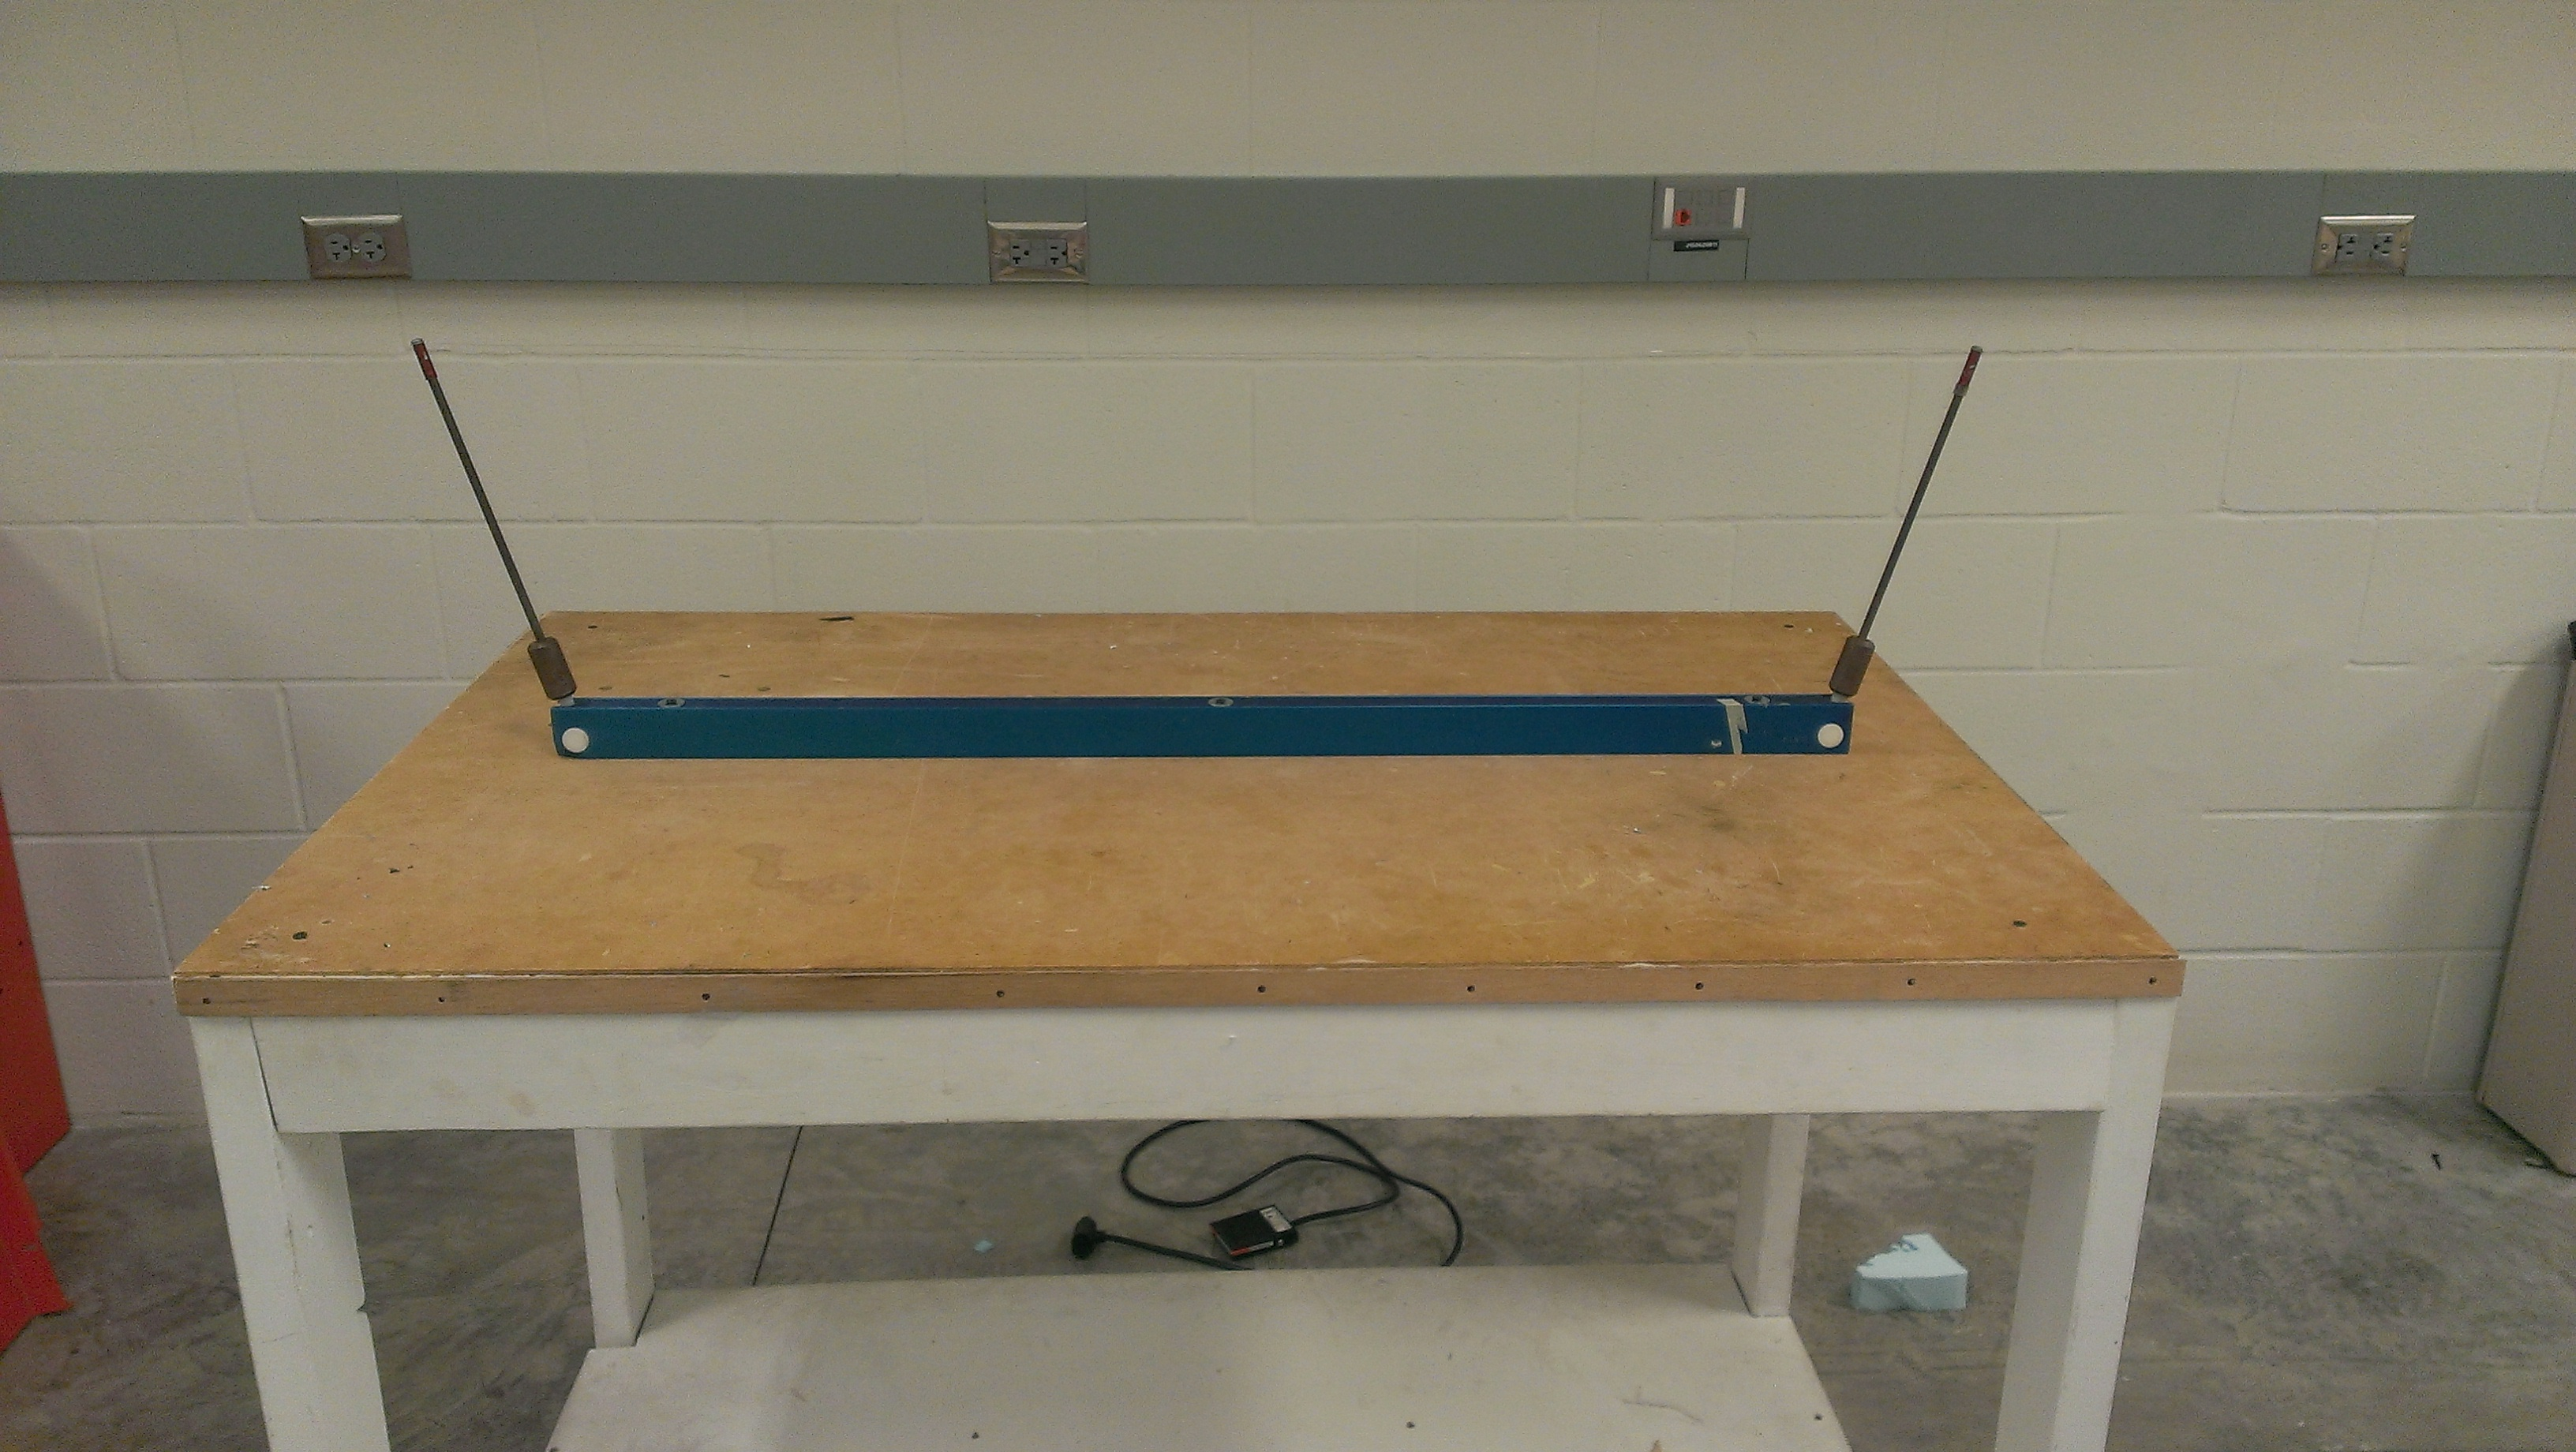
\includegraphics[width=4in]{images/IMAG0208}
\caption{Horizontal Hot Wire Cutter}
\label{fig:hortcutter}
\end{figure}

\subsection{Setup}
\begin{enumerate}
\item Ensure the hotwire is taunt, if the hotwire is not taut, loosen the top set screw and pull the wire taut and then re-tighten the set screw
\item Clip the red alligator clip to the left or right side of the wire 
\item Clip the black alligator clip to the opposite side as the red. These leads supply power to the wire
\item Plug the power unit in
\item The unit is now ready to use
\end{enumerate}
\subsection{Operation}

\begin{figure}[ht]
\centering
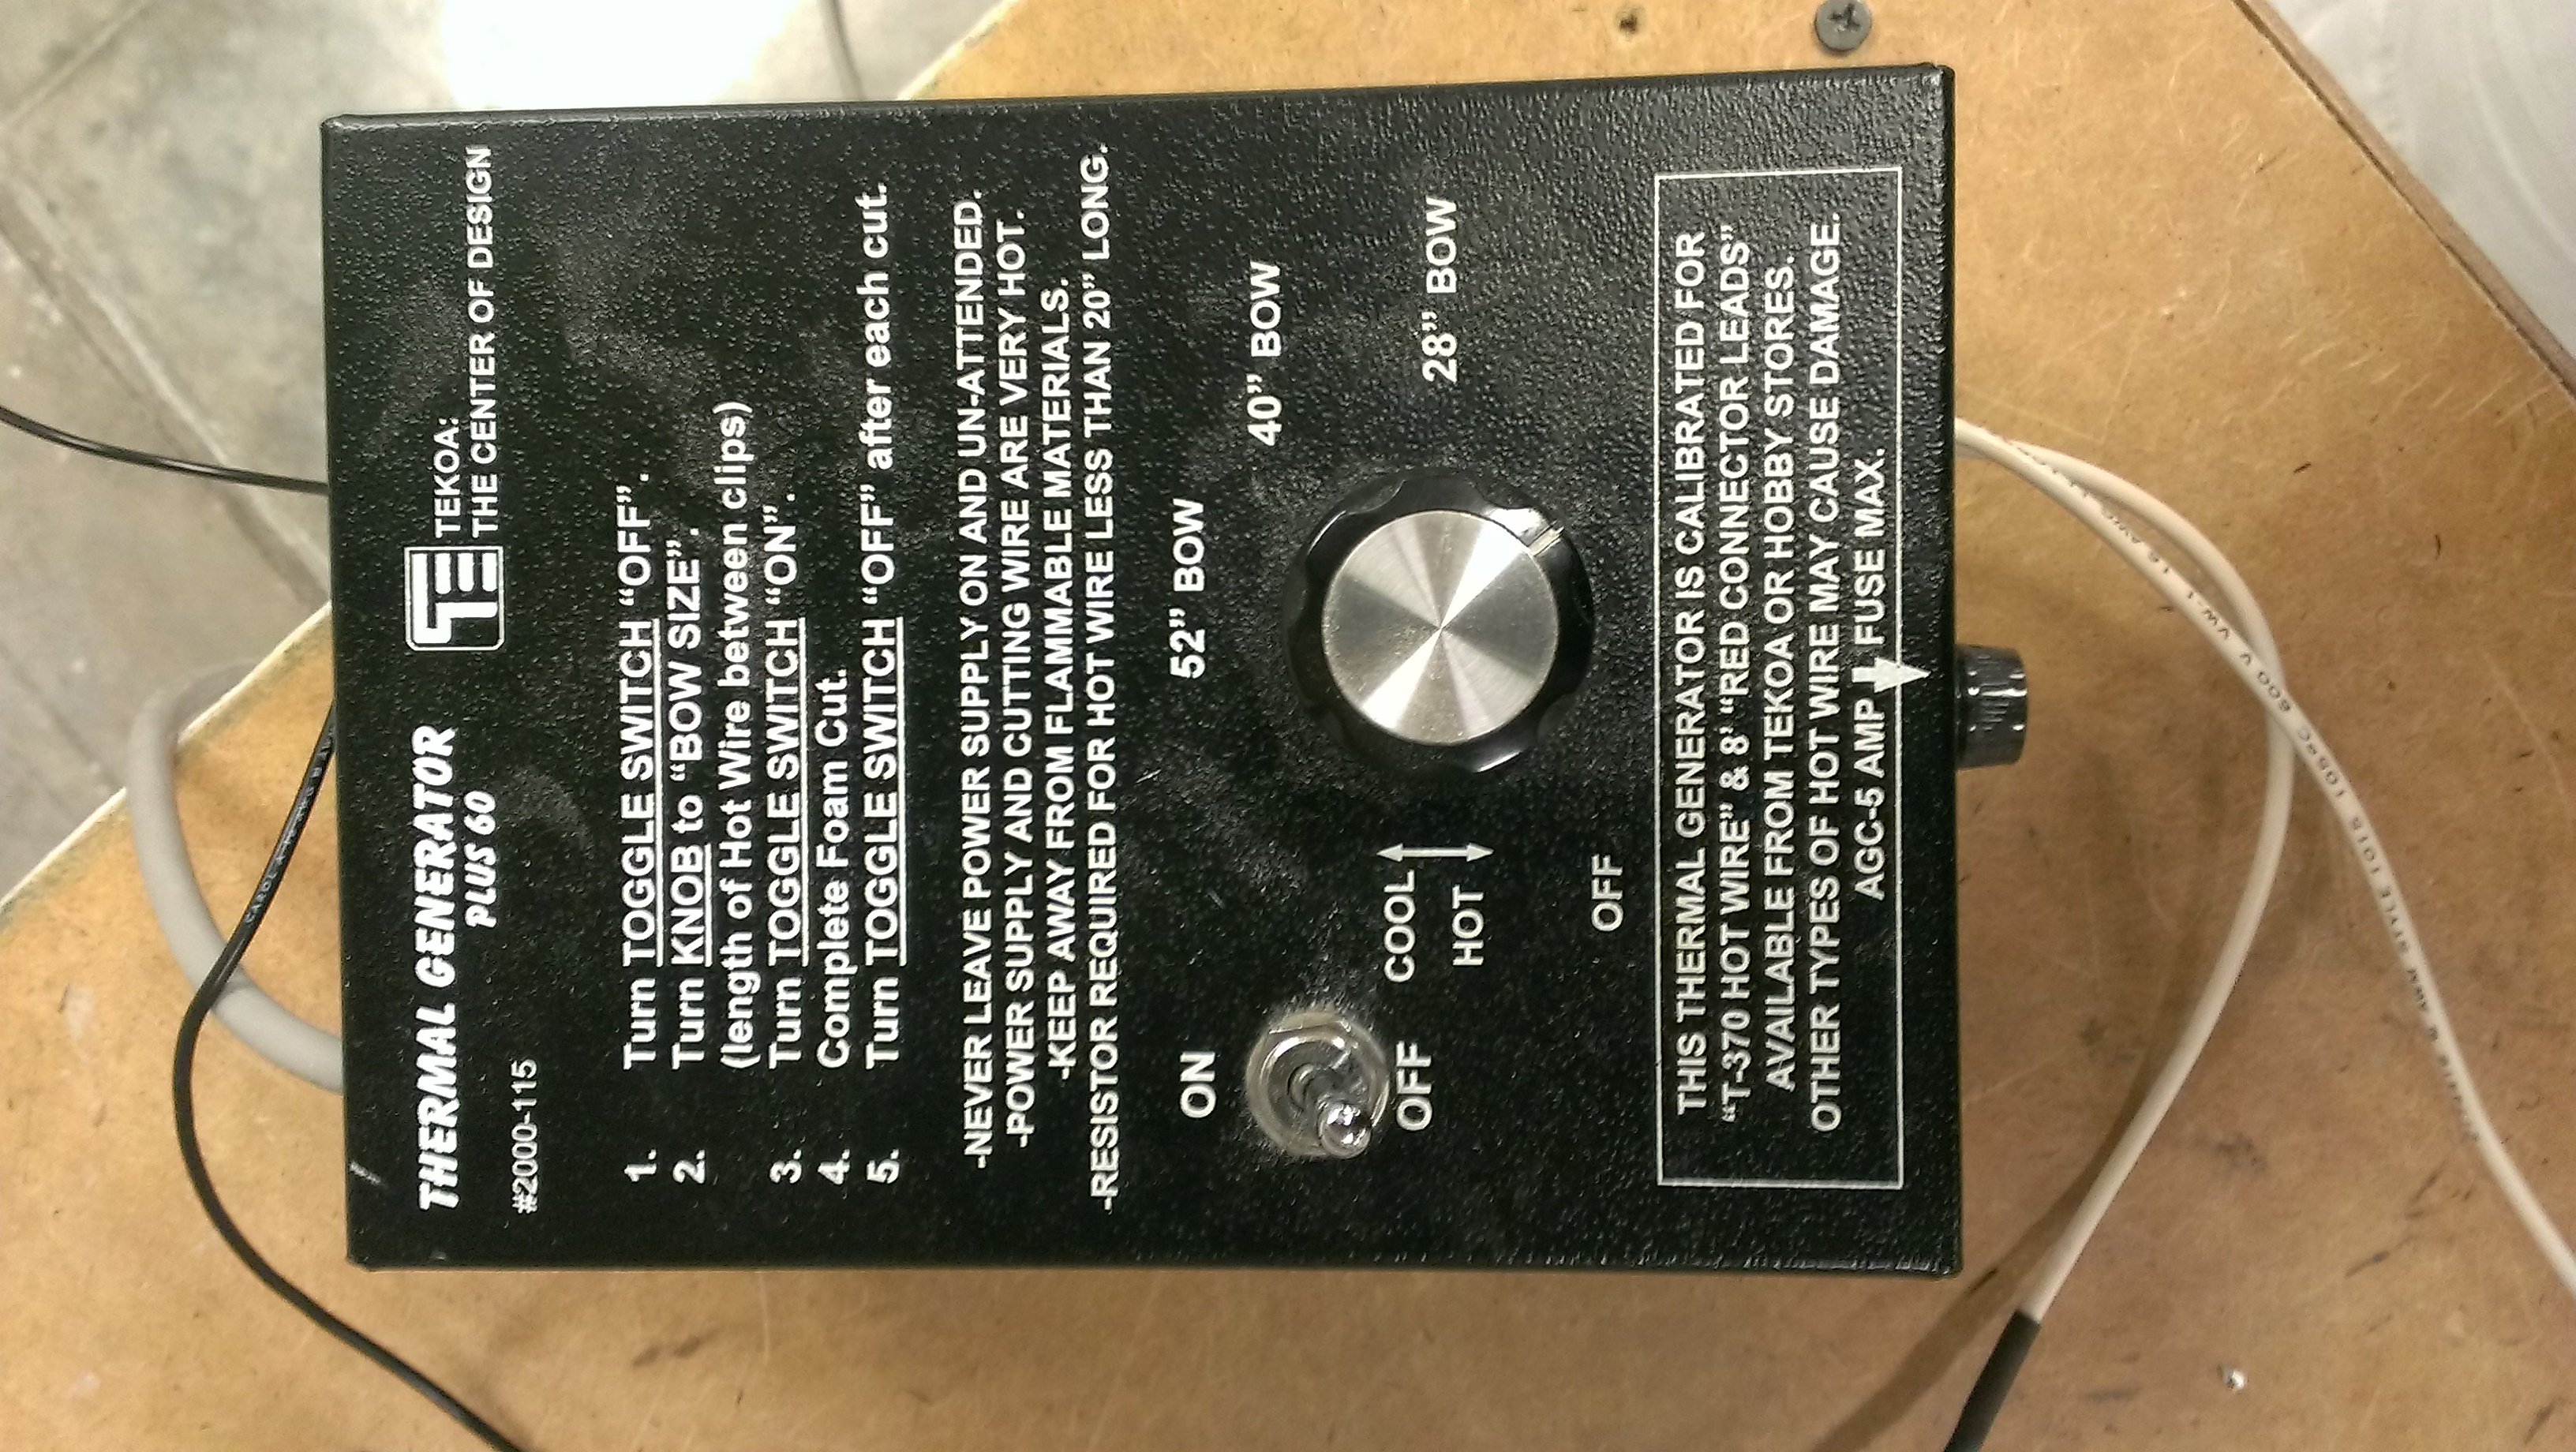
\includegraphics[angle = 270, trim = 150mm 50mm 250mm 50mm,clip,width=2in]{images/IMAG0216}
\caption{Control box for the horizontal cutter.}
\label{fig:controlbox}
\end{figure}

\begin{enumerate}
\item Set the bow size setting. This will be determined by the length of the bow itself
\item Turn the power switch into the \textbf{ON position}
\item When the wire has heated up, proceed to cut the work piece
\begin{enumerate}
\item When entering and exiting work piece, use a slow speed to prevent the wire from bowing.
\item Travel at a relatively slow pace in order to minimize wire lag
\end{enumerate}
\item When finished making cuts, turn the power off and unplug the Thermal Generator
\item Clean up immediate work area
\begin{enumerate}
\item Small, unusable foam scraps need to be thrown away
\item Excess usable foam scraps can be kept on the bottom shelf of the hot wire table
\item Sweep and vacuum after each use of the hot wire table
\end{enumerate}
\end{enumerate}

\section{Portable Hot Wire Bow}
The portable hot bow is similar in operation and purpose to the horizontal hot wire cutting station. This bow, however, it is smaller and portable.
\subsection{Setup}
\begin{enumerate}
\item Secure portable hot wire bow to an approved surface
\begin{enumerate}
\item Only the white rolling table surfaces are approved surfaces for attaching the portable hot wire
\item To secure, use two C-clamps and tighten to an exposed edge of the work surface
\end{enumerate}

\item Ensure the hotwire is taunt, if the hotwire is not taut, loosen the top set screw and pull the wire taut and then re-tighten the set screw
\item Hook up the red alligator clip of the Thermal Generator to one side of the wire and the black to the other side
\item Plug the Thermal Generator in. 
\item The portable hot wire bow is now ready to use.
\end{enumerate}
\subsection{Operation}
For operation see the Operation section of the Horizontal Hot Wire Cutting Station.
\section{Hot Knife}
Another tool for cutting foam is the hot knife which is shown in Figure \ref{fig:hotknife}. This tool operates similarly to the hot wire cutters in that it heats up a piece of metal that melts the foam. The difference is that this is a hand held tool and allows for many different complex cuts to be made.

\begin{figure}[ht]
\centering
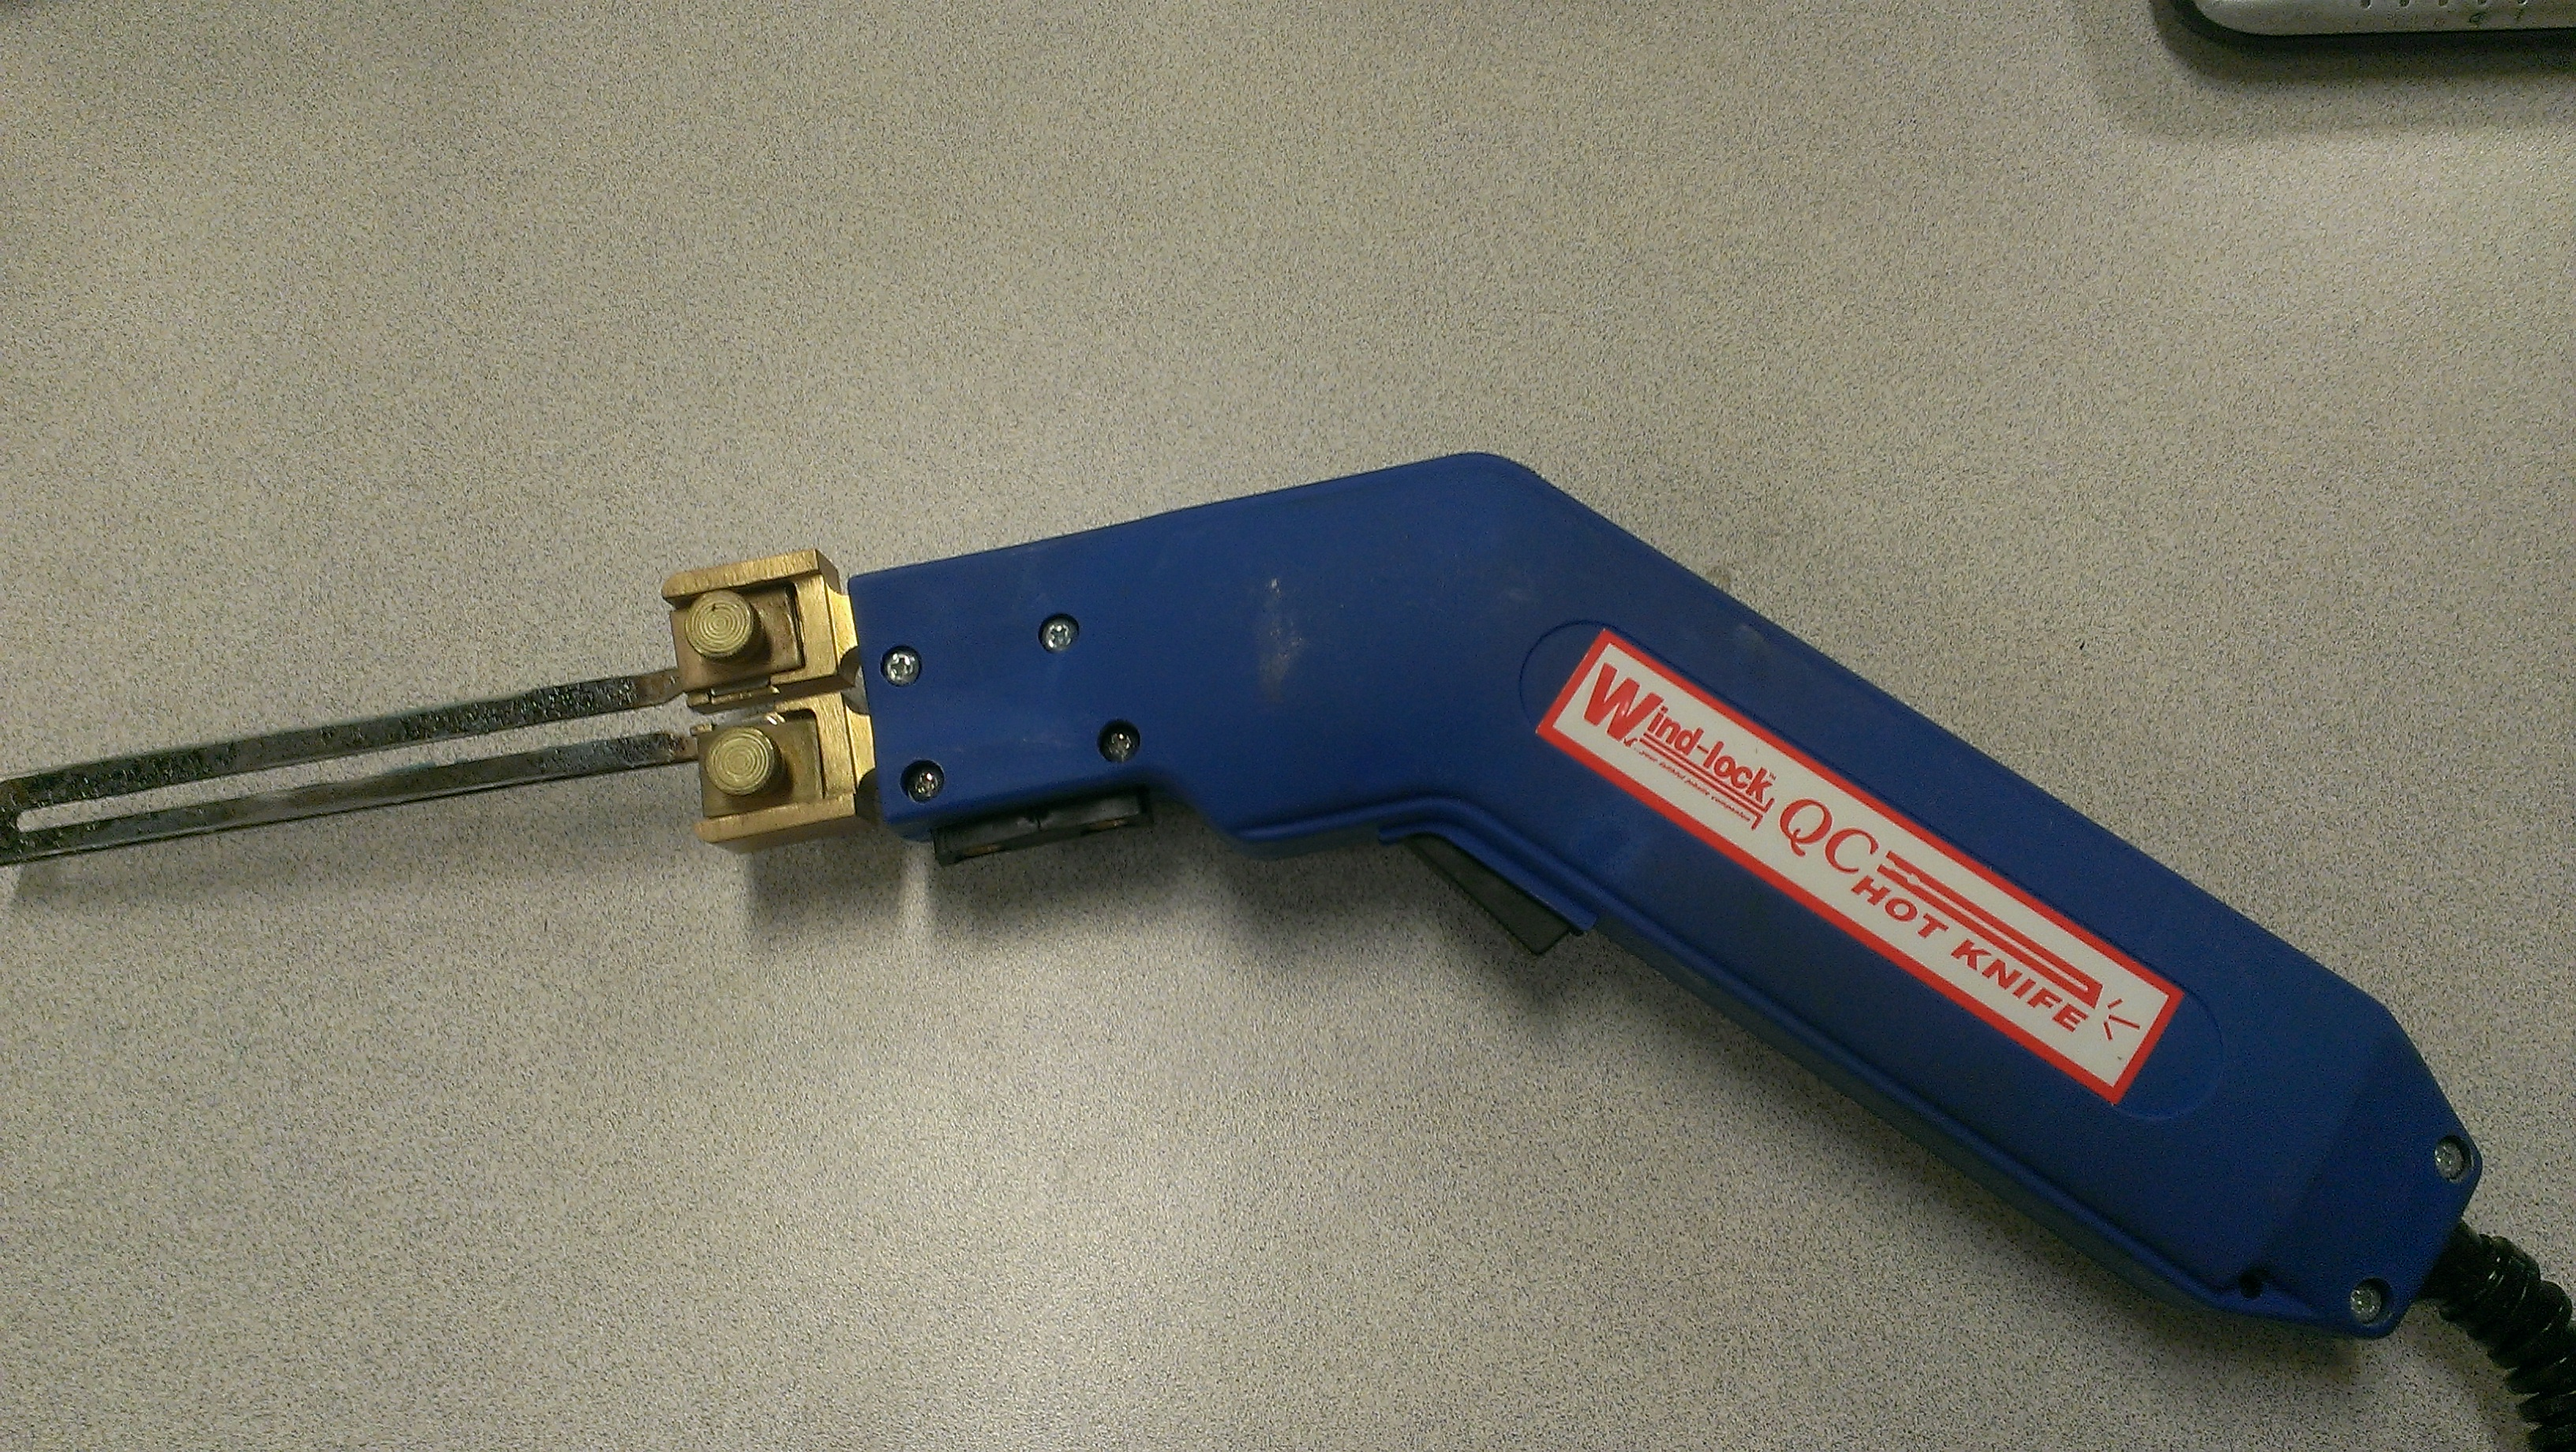
\includegraphics[width=4in]{images/IMAG0229}
\caption{Handheld hot knife}
\label{fig:hotknife}
\end{figure}

To begin using the hot knife, verify that the blade is inserted into the holder and properly secured.  In order to attach the blade, loosen the set screws, seat the blade in the grooves provided, and then tighten the set screws again.  The image below shows the blade properly seated in the hot knife.

%\begin{figure}[h]
%\centering
%\includegraphics[width=2in]{../images/IMAG0230}
%\caption{Proper seating of the blade in the hot knife.}
%\label{fig:hotwireblade}
%\end{figure}

\subsection{Basic Operation}\label{hotknife_ops}
Once the blade is secure, plug the hot knife into the outlet.  To operate the knife, press and hold the trigger.  Anytime the trigger is pulled in, the blade will quickly heat up.  Once the trigger is released, the blade will cool down.

There are two basic methods of cutting with the hot knife.  The first is to set the heat so that based off of travel rate and material, the knife cuts correctly while holding down the trigger.  The second and easier way is to turn the heat all the way up and then toggle the trigger on and off in order to achieve the desired heat in the blade.

When exiting the material, set the heat lower on the last inch or two of material so that the blade takes a bit more effort to cut with. This allows the last inch or two of material to clean off the blade of excess residue.  You should never cut with excessive heat.  Excessive heat leads to less precise cuts and also builds up melted material on the blade which ruins the blade.

When you have finished cutting your foam, ensure the blade is clean and cooled before storing.  Clean up the area immediately after done cutting and throw away any scraps.  Put away any useful pieces of foam in the proper storage area.  Vacuum and sweep up all dust and small particles that may have been generated during cutting.
\subsection{Sled Operation}

%\begin{figure}[h]
%\centering
%\includegraphics[width=2in]{../images/IMAG0233}
%\caption{The sled that may also be used with the hot knife}
%\label{fig:hotsled}
%\end{figure}
Along with the regular blade, the hot knife also comes with a sled that can make cutting straight, constant depth grooves very easy.  To use this sled, follow these steps:

\begin{enumerate}
\item Remove the blade or custom wire attachment from the hot knife.
\item Unscrew the set screws and pull the blade out.
\item Insert the sled attachment into the set screws.
\item Loosen the set screws until the attachment slides in.
\item Ensure the square metal tabs are in the correct orientation and then tighten the set screws.
\item Loosen the set screws on the front of the sled and remove the short section of custom wire.
\item Bend custom wire section to the desired profile shape and then put back into the set screw slots.
\item Tighten the set screws on the front of the sled.
\item Plug in the hot knife.
\end{enumerate}

Cutting is done in the same way as operating the hot knife with the blade attachment. See Section \ref{hotknife_ops} on cutting instructions.  Ensure the sled attachment slides evenly on the foam surface and remains in contact with the foam at all times while cutting.  When complete, ensure the blade is clean and cooled before storing.  Remove sled attachment by reversing the order used to attach it.
Make sure you clean up area immediately after done cutting and throw away scraps.  Useful pieces of foam should be properly stowed.  Vacuum and sweep the area to finish cleaning the area up.  

\subsection{Custom Wire Operation}
The hot knife cutter has another, flexible wire that allows for custom shapes to be formed.  To use the custom wire, follow the procedures below.

\begin{enumerate}
\item Bend the flexible wire into desired shape.  Avoid sharp corners and tight bends as this can ruin the wire.
\item Hook the wire into the same slots the blade attaches to.
\item Loosen set screws, attach the blade into the slots, and then tighten the set screws.
\item Plug the hot knife into an outlet.
\end{enumerate}
To operate the knife, press and hold the trigger.  There are two basic methods of cutting with the hot knife
The first is to set the heat so that based off of travel rate and material, the knife cuts correctly while holding down the trigger.

The second and easier way is to turn the heat all the way up and then toggle the trigger on and off in order to achieve the desired heat in the wire.  When exiting material, set the heat lower on the last inch or two of material so that the blade takes a bit more effort to cut with. This allows the last inch or two of material to clean off the wire of excess residue.

When using the hot knife or hot wire, never cut with excessive heat.  Excessive heat leads to less precise cuts.  Excessive heat also builds up melted material on the wire which ruins the wire.  When complete, ensure the wire is clean and cooled before storing.  When done make sure you clean up area immediately after done cutting.

\section{Sanding Foam}
\subsection{Downdraft Table}
Groups that need to sand can do so on the provided downdraft table. All sanding must be done on the downdraft table.
\begin{enumerate}
\item Turn the power switch, the left hand switch labeled power, into the ON position
\item Select the desired speed on the right hand switch labeled Speed. The up position is HIGH and the down position is LOW
\item Sand on the top surface of the machine.
\item If dust is not being pulled into the machine
\begin{enumerate}
\item Change the speed setting to HIGH if it is not already
\item If the speed is on HIGH and the dust is still not being collected, consult a lab monitor, the filter may be in need of replacement.
\end{enumerate}
\item When finished sanding, sweep any remaining dust into the collection \item system prior to turning the power off
\item Turn the power switch into the OFF position
\item Clean up the immediate area
\end{enumerate}

\subsection{Sanding Procedures}
When using procedures like CNC milling and even hot wire cutting, small defects in the material may be left over from the material removal process. In order to create a smooth, uniform finish that foam coatings can adhere to it may be necessary to sand the workpiece.  To do this, follow the steps below.

\begin{enumerate}
\item Select a sandpaper grit.  Generally 100 or 150 grit sandpaper is sufficient to sand foam.
\item Sand the foam until it reaches its desired shape.
\end{enumerate}

Since foam is much softer than wood, sanding will take much less time and require less effort to sand.  Rarely will it be necessary to sand foam with sandpaper of a higher grit than 150.  For most applications, one grit should be sufficient, however for finer finishes it may be beneficial to use a second grit.

\chapter{Foam Coatings}
Groups may want to cover their foam projects in a protective layer. There are several coatings available to students that can offer increased rigidity, strength, or flexibility.
\section{Composites}
The Make to Innovate lab has access to composite materials like fiberglass and carbon fiber. Groups are able to use these materials on their projects if needed, however, there may be a cost associated with these materials.  In addition, all composites work must take place in 0638 Howe Hall and additional training is required to work with composites.

\subsection{Carbon Fiber}
Carbon fiber is a composite material that students have access to use on their projects for an additional cost. Carbon fiber is an expensive material, but it is lighter and stiffer than other materials like fiberglass. There are certain situations in which carbon fiber is an appropriate material, despite its higher cost. Projects that require a larger strength to weight ratio and more stiffness could make use of carbon fiber. Most projects, however, do not need the benefits that carbon fiber provides. Fiberglass is a perfectly suitable material for most situations.

Groups who wish to use carbon fiber need to first seek out the approval of the use of the composites lab materials from Matthew Nelson. Upon approval, students can go to the composites lab and speak to the composites lab monitor. The lab monitor will be able to point out all necessary training that needs to be completed before using the composites lab. The monitor will also be able to educate students on how best to go about coating their project in carbon fiber.

\subsection{Fiberglass}
Fiberglass is a composite coating that is relatively cheap and relatively strong. Students have access to use this material for their projects and depending on availability it may be available at no cost to the team. For most projects, fiberglass is more than sufficient to add stiffness and strength. 

In order to use fiberglass, students must get approval from Matthew Nelson prior to being able to use lab supplies. If approved, students must then seek out the help of the composites lab monitor. The composites monitor will point out all necessary training that needs to be completed as well as the best practices on how to do their composites work.

\section{Foam Coat}
Foam coat is a new material that the lab is experimenting with. It is a gypsum coating that, depending on the additive, can add strength and flexibility. This coating is water based and can be cleaned up with water, making it easier to use and less dangerous than traditional foam coatings. There are several different additives that change the properties of the foam coat. If groups want to experiment with foam coat, they can speak with a lab monitor who will help them out.

\subsection{Base Mix}
The base mix is gypsum and water that can be mixed in various thicknesses. If thinner applications are desired, more water can be added to allow for easy spreading. Thicker applications require less water and allow for a stickier coating. For complete mixing instructions, read the label and instructions.
\subsection{Boost}
Boost, when mixed in the appropriate quantities, strengthens the base material and allows for thinner applications. This means lighter overall weight and higher strength. This coating is relatively brittle and will crack if flexed much. For mixing instructions, read the label and follow directions.
\subsection{Bounce}
When mixed in the base mix, bounce creates a flexible, rubbery coating that resists cracking. This coat does not add much rigidity, but is weather resistant. For mixing instructions, please refer to the label on the product.
\subsection{Best Coating}
The best option that has been explored so far utilizes both the boost mix and the bounce mix.  Please follow the steps below for doing a best coast method.

\begin{enumerate}
\item Prepare the surface for finishing.  All cutting, sanding, and surface prep. must be done prior to coating.
\item Mix a batch of the boost material.
\item Apply the boost material in a uniform coating.  Thickness will depend on the desired strength and weight.
\item Let coating dry completely.
\item Mix a batch of bounce.
\item Apply a coat of bounce to the piece on top of the dried coat of boost.
\end{enumerate}
Thickness will depend on the desired flexibility and weight.  Layering the two coats of material will allow for a strong, flexible part.  When bent, the boost layer may crack, but the bounce layer will stretch and contain the boost.

\section{Paint}
Painting is cheap and effective way to enhance the appearance of a project. Painting foam, however, can be difficult. Spray paints and certain other paints have solvents that will also dissolve the foam. The best way to paint foam is to use water or latex based brush-on paint. The lab has these paints readily available for student use. See a lab monitor for access to the paints.


%\newthought{The pages} of a book are usually divided into three major sections: the front matter (also called preliminary matter or prelim), the main matter (the core text of the book), and the back matter (or end matter).



%%
% The back matter contains appendices, bibliographies, indices, glossaries, etc.


\backmatter

% \bibliography{sample-handout}
% \bibliographystyle{plainnat}


\printindex

\end{document}
